\documentclass[11pt,twoside]{article}

\usepackage[margin=1in]{geometry}
\usepackage{amsmath,amssymb,amsthm,mathtools}
\usepackage{thmtools}
\usepackage[inline,shortlabels]{enumitem}
\usepackage{booktabs}
\usepackage{xcolor}
\usepackage{microtype}
\usepackage{tikz}
\usepackage{pgfplots}
\pgfplotsset{compat=1.18}
\usetikzlibrary{arrows.meta,positioning,calc}

% Revision date: maintained by scripts/build_lecture_notes.py. Keep this command.
\newcommand{\lecturerevised}{2026-09-15 23:22 UTC-06:00}
\usepackage{eso-pic}
\AddToShipoutPictureBG{%
  \AtPageLowerLeft{%
    \put(\LenToUnit{0.5\paperwidth},\LenToUnit{0.5in}){%
      \makebox(0,0){\normalfont\footnotesize\color{black!60}Last revised: \lecturerevised}%
    }%
  }%
}
\usepackage[square,authoryear]{natbib}
\usepackage{xr-hyper}
\usepackage[colorlinks=true,linkcolor=blue!60!black,
  urlcolor=blue!60!black,citecolor=blue!60!black]{hyperref}
\usepackage[nameinlink,capitalize]{cleveref}
\hypersetup{pdftitle={Lecture 5: State-space models and system identification},
  pdfauthor={Csaba Szepesvari}}
\crefname{exercise}{Exercise}{Exercises}
\Crefname{exercise}{Exercise}{Exercises}

\usepackage{enotez}
\DeclareInstance{enotez-list}{lecture}{list}{format=\normalsize,number={#1.}}
\setenotez{list-name=Endnotes,list-style=lecture,backref=true}
\crefname{endnote}{Endnote}{Endnotes}
\Crefname{endnote}{Endnote}{Endnotes}

\definecolor{courseblue}{HTML}{17365D}
\tikzset{
 ssm flow/.style={-Latex,line width=.85pt,draw=courseblue},
 ssm block/.style={draw=courseblue,line width=.85pt,rounded corners=1.5pt,
   fill=courseblue!3,minimum width=24mm,minimum height=12mm,align=center},
 ssm delay/.style={draw=courseblue,line width=.85pt,fill=white,
   minimum width=17mm,minimum height=11mm,align=center,font=\small},
 pics/ssm noise/.style={code={
   \draw[courseblue,line width=.85pt,fill=white] (-.34,-.34) rectangle (.34,.34);
   \fill[orange!85!black] (.08,.25)--(-.17,-.025)--(-.015,-.025)
      --(-.10,-.26)--(.18,.065)--(.035,.065)--cycle;
 }},
 pics/ssm eye/.style={code={
   \draw[courseblue,line width=.85pt,fill=white]
     (-.43,0) .. controls (-.16,.30) and (.16,.30) .. (.43,0)
     .. controls (.16,-.25) and (-.16,-.25) .. (-.43,0);
   \fill[courseblue] (0,0) circle (.085);
   \draw[courseblue,line width=.85pt]
     (-.31,.12)--(-.42,.27) (-.16,.20)--(-.21,.38)
     (.16,.20)--(.21,.38) (.31,.12)--(.42,.27);
 }}
}
\newcommand{\R}{\mathbb R}
\newcommand{\E}{\mathbb E}
\newcommand{\I}{\mathbb I}
\renewcommand{\P}{\mathbb P}
\newcommand{\KL}{D}
\newcommand{\TV}{\mathrm{TV}}
\newcommand{\suppmark}{\texorpdfstring{\textsuperscript{*}}{*}}
\DeclareMathOperator{\diag}{diag}
\DeclareMathOperator{\rank}{rank}
\makeatletter
\@for\@letter:=A,B,C,D,E,F,G,H,I,J,K,L,M,N,O,P,Q,R,S,T,U,V,W,X,Y,Z\do{%
  \expandafter\edef\csname c\@letter\endcsname{\noexpand\mathcal{\@letter}}}
\makeatother
\newtheorem{theorem}{Theorem}[section]
\newtheorem{proposition}[theorem]{Proposition}
\newtheorem{corollary}[theorem]{Corollary}
\theoremstyle{definition}
\newtheorem{definition}[theorem]{Definition}
\newtheorem{example}[theorem]{Example}
\theoremstyle{remark}
\newtheorem{remark}[theorem]{Remark}
\renewcommand{\thepage}{5--\arabic{page}}
\renewcommand{\thesection}{5.\arabic{section}}
\renewcommand{\theequation}{5.\arabic{equation}}
\pagestyle{myheadings}
\markboth{Lecture 5: State-space models and system identification}
{Lecture 5: State-space models and system identification}
\usepackage{../exercises/course-exercises}

\begin{document}

\begin{center}
\fcolorbox{courseblue}{white}{%
\begin{minipage}{0.92\textwidth}
\vspace{1mm}
\textbf{CMPUT 654: Mathematical Foundations of Modern AI Systems}
\hfill Fall 2026
\vspace{3mm}
\begin{center}
{\Large\bfseries Lecture 5: State-space models and system identification}
\vspace{1mm}

September 15, 2026
\end{center}
\vspace{2mm}
\textit{Lecturer: Csaba Szepesv\'ari}
\hfill
\textit{Note prepared by: Csaba Szepesv\'ari}
\vspace{1mm}
\end{minipage}}
\end{center}

\noindent\textbf{About these lecture notes.}
This lecture asks how a structured hidden state can explain a sequence,
how to predict and generate after observing a prefix, and how to fit the
model from observations. The main construction first fits observed lag
coefficients, then recovers a compact recurrent predictor by matrix
factorization.

\medskip
\noindent\textbf{Scope and reading guide.}
The main text follows the classroom sequence: nonlinear state-space
models, conditional generation, estimation and identifiability, latent
likelihoods and EM, observable prediction, linear models, and the
subspace algorithm. It develops the questions about memory, parameter
sharing, backpropagation, and attention raised in class.
The synthetic comparisons are additions to the lecture.
The optional section after this development justifies the algorithm and
relates estimation error to prediction, sequence KL, and generation.
Cayley--Hamilton was not presented in class; it is retained as an optional
noiseless comparison and an exercise. After the take-home messages, the notes
continue with endnotes, bibliographical notes and references, the glossary,
exercises, and appendices.

\medskip
\noindent\textbf{Notation.}
States are \(S_t\in\cS\), observations are \(Z_t\in\cZ\), and
\(Z_{<t}=Z_{1:t-1}\). Finite observation labels are denoted \(X_t\).
Vectors are columns. \(T\) is trajectory length; \(d\) and \(m\) are
state and observation dimensions. Expectations refer to the model law
specified at their use; logarithms are natural.
Lecture~4 supplies the sequence KL and recovery background.
Superscript asterisks\suppmark{} mark optional material; numbered endnotes
contain short refinements.

\section{State, observations, and the modeling choice}
\label{sec:state-space}

A state-space model specifies what information a process retains and how
that information produces observations. Let \(\cS\) and \(\cZ\) be the
state and observation spaces. We use the equations
\begin{equation}
 S_0\sim\pi_\theta,\qquad
 S_{t+1}=f_\theta(S_t,V_{t+1}),\qquad
 Z_{t+1}=g_\theta(S_{t+1},W_{t+1}),\quad t\ge0.
 \label{eq:nonlinear-ssm}
\end{equation}
Here \((V_t)_{t\ge1}\) and \((W_t)_{t\ge1}\) are independent iid
sequences, independent also of \(S_0\). Their laws are part of the model
and may depend on \(\theta\). The two noise laws need not be the same.
We assume measurable update maps; Euclidean spaces and finite sets cover
our examples.\endnote{\textbf{General spaces.}
Standard Borel spaces suffice for the conditional distributions and
randomized kernel representations used here. An arbitrary measurable
space need not have these properties.}

\begin{figure}[htbp]
\centering
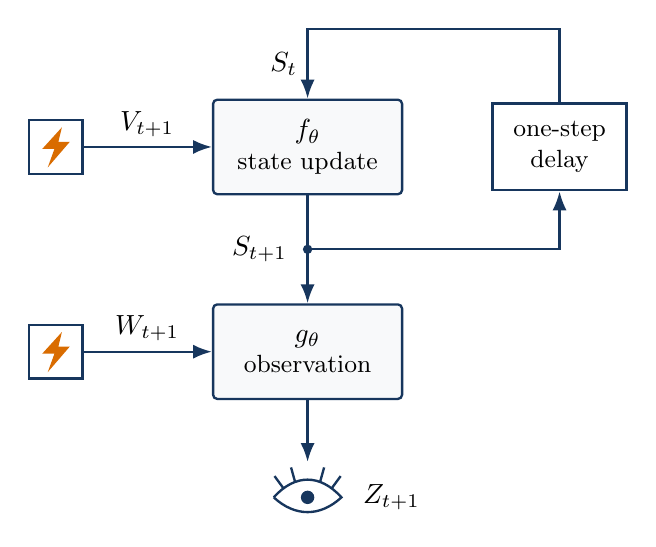
\begin{tikzpicture}[font=\normalsize]
\node[ssm block] (f) at (0,2.6) {$f_\theta$\\[-1pt]\small state update};
\node[ssm block] (g) at (0,0) {$g_\theta$\\[-1pt]\small observation};
\node[ssm delay] (memory) at (3.2,2.6) {one-step\\delay};
\pic at (-3.2,2.6) {ssm noise};
\pic at (-3.2,0) {ssm noise};
\draw[ssm flow] (-2.86,2.6)--node[above]{$V_{t+1}$}(f.west);
\draw[ssm flow] (-2.86,0)--node[above]{$W_{t+1}$}(g.west);
\coordinate (state) at (0,1.3);
\draw[courseblue,line width=.85pt] (f.south)--(state);
\draw[ssm flow] (state)--(g.north);
\fill[courseblue] (state) circle (1.7pt);
\node[left=4pt] at (state) {$S_{t+1}$};
\draw[ssm flow] (state)--(3.2,1.3)--(memory.south);
\draw[ssm flow] (memory.north)--(3.2,4.1)--(0,4.1)
 --node[left]{$S_t$}(f.north);
\draw[ssm flow] (g.south)--(0,-1.40);
\pic at (0,-1.85) {ssm eye};
\node[right] at (.58,-1.85) {$Z_{t+1}$};
\end{tikzpicture}
\caption{A state-space model. Independent noise sources enter the update
and observation maps. The state feeds both the observation map and the
next update; the one-step delay is initialized with \(S_0\).
Dots mark branches of the same signal. The eye marks the observed output.}
\label{fig:ssm}
\end{figure}

The process \((S_t)\) is Markov: conditional on its current state, its
next state does not depend on earlier states or observations.
We call the full construction a \emph{hidden Markov model} (HMM), and
\((Z_t)\) its \emph{observation process}, or a \emph{hidden Markov process}.
The pair process \((S_t,Z_t)_{t\ge1}\) is Markov. The observation process
alone generally is not. We will say \emph{finite HMM} when \(\cS\) is
finite. This terminology also allows a continuous-state HMM.

\subsection{Where the inductive bias enters}

The useful assumption is a small or structured state space and a
restricted update rule. As in Lecture~1, an architecture relates
predictions at different inputs through shared structure.
For physical motion, a few state coordinates can have known meanings.
For language, identifying a useful compact state is itself a learning
problem.

With unrestricted state space and maps, the state can record the entire
history. More precisely, it can store a finite observation string,
sample its next symbol from the desired conditional law, append that
symbol, and emit it. The string includes its length, so this construction
can also describe a process whose conditional law changes with time.
It gives a state-space representation of any process with the required
conditional distributions. The growing state supplies no compression
or structural restriction.

The representation is a modeling choice. Removing process noise gives
\[
 S_{t+1}=f_\theta(S_t),\qquad Z_t=g_\theta(S_t,W_t).
\]
All state randomness then comes from the initial state. Another choice
computes a predictor's state from observed feedback:
\begin{equation}
 R_{t+1}=h_\theta(R_t,Z_t),\qquad
 Z_t=j_\theta(R_t,W_t),\qquad R_1=r_\theta.
 \label{eq:observation-driven}
\end{equation}
Given a prefix, \(R_t\) is known. During generation, random observations
feed randomness into future states.

\begin{figure}[htbp]
\centering
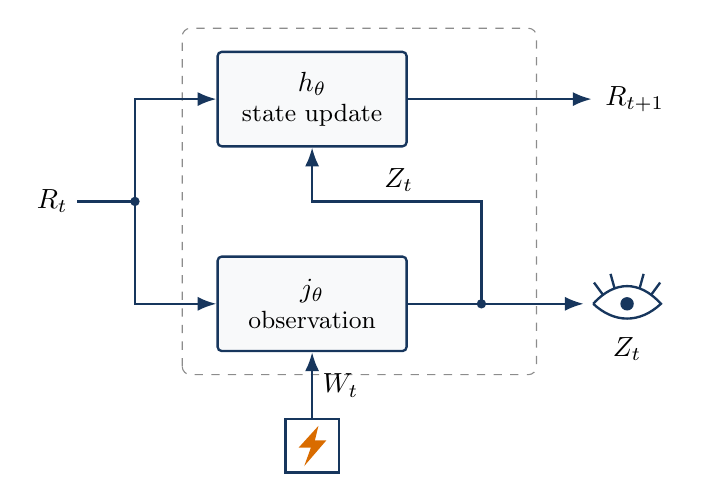
\begin{tikzpicture}[font=\normalsize]
\draw[dashed,black!45,rounded corners=3pt]
 (-1.65,-.9) rectangle (2.85,3.5);
\node[ssm block] (h) at (0,2.6) {$h_\theta$\\[-1pt]\small state update};
\node[ssm block] (j) at (0,0) {$j_\theta$\\[-1pt]\small observation};
\node (current) at (-3.3,1.3) {$R_t$};
\coordinate (state) at (-2.25,1.3);
\draw[courseblue,line width=.85pt] (current.east)--(state);
\fill[courseblue] (state) circle (1.7pt);
\draw[ssm flow] (state)--(-2.25,2.6)--(h.west);
\draw[ssm flow] (state)--(-2.25,0)--(j.west);
\draw[ssm flow] (h.east)--(3.55,2.6);
\node[right] at (3.6,2.6) {$R_{t+1}$};
\coordinate (observed) at (2.15,0);
\draw[courseblue,line width=.85pt] (j.east)--(observed);
\fill[courseblue] (observed) circle (1.7pt);
\draw[ssm flow] (observed)--(2.15,1.3)--(0,1.3)--(h.south);
\node[above] at (1.1,1.3) {$Z_t$};
\draw[ssm flow] (observed)--(3.45,0);
\pic at (4,0) {ssm eye};
\node[below] at (4,-.3) {$Z_t$};
\pic at (0,-1.8) {ssm noise};
\draw[ssm flow] (0,-1.46)--node[right]{$W_t$}(j.south);
\end{tikzpicture}
\caption{One step of an observation-driven model. First, \(R_t\) and the
observation noise produce \(Z_t\). Then \(R_t\) and \(Z_t\) produce
\(R_{t+1}\), which is carried to the following step. Dots split one signal
into two branches. The dashed enclosure does not eliminate the state
carried between steps, so \(Z_t\) need not be Markov.}
\label{fig:observed-feedback}
\end{figure}

The pair \((R_t,Z_t)\) is Markov, but observing \(Z_t\) need not reveal
\(R_t\). Only an additional restriction, such as
\(Q_\theta(Z_{t+1}\in\cdot\mid Z_{1:t})
 =Q_\theta(Z_{t+1}\in\cdot\mid Z_t)\), makes the observations
first-order Markov. \Cref{ex:l5-feedback} gives a small counterexample.
This resolves the question raised by drawing one large box around the
two computations: one must still specify what the box stores and what
is observed.

\subsection{The equations define a probability law}
\label{sec:model-law}

The initial law, noise laws, and maps together determine a unique law
\(Q_\theta\) on state and observation sequences. Define the transition
and emission kernels
\[
 a_\theta(s,B)=\P(f_\theta(s,V_1)\in B),\qquad
 b_\theta(s,D)=\P(g_\theta(s,W_1)\in D).
\]
Their joint law has the product form
\begin{equation}
 Q_\theta(ds_{0:T},dz_{1:T})
 =\pi_\theta(ds_0)\prod_{t=1}^T
 a_\theta(s_{t-1},ds_t)b_\theta(s_t,dz_t).
 \label{eq:ssm-joint}
\end{equation}
A density or probability-mass version uses products of transition
and emission densities or masses. A general kernel need not have a density.

The correspondence is not one-to-one. Different randomized maps can
implement the same kernels; different hidden representations can give
the same observation law.

For a finite HMM, let \(S_t\in[d]\) and \(X_t\in[N]\), with
\[
 A_{ij}=Q_\theta(S_t=i\mid S_{t-1}=j),\qquad
 C_{aj}=Q_\theta(X_t=a\mid S_t=j).
\]
Both matrices are column-stochastic, matching column-vector probability
distributions. With \(\pi_j=Q_\theta(S_0=j)\),
\begin{equation}
 Q_\theta(s_{0:T},x_{1:T})
 =\pi_{s_0}\prod_{t=1}^T A_{s_ts_{t-1}}C_{x_ts_t}.
 \label{eq:hmm-joint}
\end{equation}
Independent uniform random variables and inverse cumulative sums of the
columns implement \(f_\theta,g_\theta\); \cref{ex:l5-kernels} asks for
the construction. Here \(X_t\) is the discrete observation label;
later \(Z_t=e_{X_t}\) is its vector encoding.

\section{Generation after an observed prefix}
\label{sec:filtering}

Unconditional generation follows the equations: sample \(S_0\), then
sample fresh noises at each step. Conditional generation must first
account for what the observations reveal about the hidden state.

Let
\[
 \mu_t^-=Q_\theta(S_t\in\cdot\mid Z_{<t}=z_{<t})
\]
be the \emph{predictive state distribution}. To sample a continuation
\(Z_{t:T}\), first sample \(S_t\sim\mu_t^-\), then sample \(Z_t\)
from its emission kernel. Continue with the transition to \(S_{t+1}\)
and the remaining emissions. Starting instead by applying the
state update would skip the observation at time \(t\).

After seeing \(z_t\), Bayes' rule gives the \emph{filtering distribution}
and the next prediction:
\begin{equation}
 \mu_t(ds)=\frac{b_\theta(z_t\mid s)\mu_t^-(ds)}
 {\int b_\theta(z_t\mid u)\mu_t^-(du)},\qquad
 \mu_{t+1}^-(B)=\int a_\theta(s,B)\mu_t(ds).
 \label{eq:filter}
\end{equation}
This notation assumes an emission density or mass and a positive
denominator. Conditional laws are specified only almost surely.

For a finite HMM, \(\alpha_0=\pi\) and
\begin{equation}
 \alpha_t^-=A\alpha_{t-1},\qquad
 \alpha_t=\frac{\diag(C_{x_t,1},\ldots,C_{x_t,d})\alpha_t^-}
 {\mathbf1^\top\diag(C_{x_t,1},\ldots,C_{x_t,d})\alpha_t^-}.
 \label{eq:hmm-filter}
\end{equation}
Each step costs \(O(d^2)\) for dense \(A\). This is the forward
filtering recursion. Viterbi instead finds a most likely complete
hidden path; smoothing computes posterior state distributions using
observations on both sides of the time in question.

For continuous nonlinear models, \emph{particle filtering} approximates
the filtering distribution by weighted sampled states: propagate particles
through the transition, weight them by observation likelihood, and
resample when needed. It requires more than a simulator for an arbitrary
observation map: the usual bootstrap filter needs evaluable likelihood
weights. Stability and forgetting can prevent errors from accumulating,
but dynamical stability alone is not a sufficient general theorem.
Observation informativeness, mixing, dimension, and the particle count
also matter; the bibliographical notes give precise sources.
A Gaussian linear model permits exact filtering with means and covariances.

\section{What can be learned from observations?}
\label{sec:estimation}

If finite hidden states were observed, transition and emission counts
would give direct estimates of \(A,C\). For linear models with observed
states, least squares estimates the linear maps under standard rank
conditions. Hidden states remove these directly observed targets.

We focus on a single observed trajectory \(Z_{1:T}\). With independent
trajectories, log likelihoods add and the recursions restart at each
initial state. These are straightforward algorithmic changes; the
statistical information can be substantially different.

For example, a long mixing trajectory contains repeated information
about transitions but only one draw from its initial law. Even observing
\(S_0\) exactly would not consistently estimate an unrestricted
\(\pi_\theta\) from that one draw. Later observations do not supply
independent initial states. Mixing and excitation help estimate the
dynamics; neither manufactures new draws from \(\pi_\theta\).
Lecture~6 returns to learning from dependent data.

\subsection{Identifiability and the meaning of success}
\label{sec:identification}

Relabeling hidden states leaves a finite HMM's observation law unchanged.
Unreachable extra states, or suitably duplicated states with identical
observable behavior, can leave it unchanged too. Thus neither the state
labels nor an unrestricted state count are identifiable.

For an LDS, an invertible coordinate change \(S_t'=T_0^{-1}S_t\)
changes the matrices to
\[
 A'=T_0^{-1}AT_0,\qquad C'=CT_0
\]
and transforms the noise and initial laws accordingly. The observations
retain exactly the same distribution. Even beyond this coordinate
ambiguity, an observation law need not uniquely separate physical process
noise from measurement noise.

Three useful questions are:
\begin{enumerate}[leftmargin=*,itemsep=.2em]
\item How accurately does the model predict the next observation?
\item How close are its conditional or joint observation laws, for example
in KL, and its generated task statistics?
\item Under suitable minimality assumptions, how accurately are a predictive
realization's matrices recovered up to a change of coordinates?
\end{enumerate}
The third can help answer the first two, but the conversion needs
conditioning and stability assumptions. Small matrix error alone is
not a uniform long-horizon guarantee.

\subsection{Likelihood evaluation and optimization}
\label{sec:latent-likelihood}

The observed likelihood marginalizes the hidden trajectory. For the
finite HMM,
\begin{equation}
 Q_\theta(X_{1:T})=
 \sum_{s_{0:T}\in[d]^{T+1}}
 \pi_{s_0}\prod_{t=1}^T A_{s_ts_{t-1}}C_{X_ts_t}.
 \label{eq:hmm-likelihood}
\end{equation}
There are \(d^{T+1}\) terms with this initialization convention.
If the initial distribution is specified directly for \(S_1\),
there are \(d^T\) terms. The forward recursion evaluates the sum in
\(O(Td^2)\) arithmetic operations; normalization at each step or a
log-domain calculation prevents numerical underflow.
For continuous states, marginalization is an integral.

We fit \(\theta\) by minimizing \(-\log Q_\theta(Z_{1:T})\).
Differentiating the finite-HMM forward algorithm is feasible and is
implemented in modern software. Its reverse-mode differentiation has
the same order of arithmetic work as likelihood evaluation, with
additional storage or recomputation. It does not make the objective
convex or ensure a global optimum. A large state count remains expensive.

Monte Carlo is also used for likelihoods and gradients in nonlinear
state-space models. Sequential Monte Carlo exploits the time structure;
sampling entire trajectories independently from the prior can produce
extremely variable likelihood estimates. An unbiased likelihood
estimate does not give an unbiased log likelihood after taking its log.

\subsection{EM and optimization over hidden trajectories}
\label{sec:em}

\emph{Expectation--maximization} (EM) uses the current parameters
\(\theta^{(k)}\) to compute a posterior over hidden trajectories,
then maximizes the expected complete-data log likelihood:
\begin{align}
 q_k(ds)&=Q_{\theta^{(k)}}(ds_{0:T}\mid Z_{1:T}),\nonumber\\
 \theta^{(k+1)}&\in\arg\max_\theta
 \E_{S\sim q_k}[\log Q_\theta(S,Z_{1:T})].
 \label{eq:em}
\end{align}
For a finite HMM, forward--backward supplies expected transition and
emission counts; these replace the observed counts. For a Gaussian LDS,
the E-step uses smoothing means \emph{and second moments}, including
cross moments at adjacent times. Substituting a single estimated state
path is generally a different algorithm.

Exact EM makes the observed log likelihood nondecreasing. Under regularity
conditions its limit points are stationary; a local maximum of likelihood
is not guaranteed in general. Efficient E- and M-steps are available for
important model families, not for every nonlinear state-space model.
\Cref{ex:l5-em} asks for the monotonicity calculation.

Another approach treats the hidden states as optimization variables:
\begin{equation}
 \min_{\theta,s_{0:T}}-\log Q_\theta(s_{0:T},Z_{1:T}).
 \label{eq:joint-map}
\end{equation}
This maximizes a joint mass or density, rather than summing or integrating
over states. A prior on \(\theta\) gives a joint MAP objective.
Sparse trajectory optimization is central in smoothing and SLAM.
It can remain nonconvex. For continuous states its density objective also
depends on the chosen coordinates and reference measure.

For deterministic linear state dynamics and unit Gaussian observation
noise, optimizing the initial state \(s=S_1\) gives
\[
 \min_{A,C,s}\sum_{t=1}^T\|Z_t-CA^{t-1}s\|_2^2.
\]
Unknown quantities multiply, and powers of \(A\) appear. Deterministic
dynamics simplify marginalization without making this parameter fit convex.

The observation-driven model in \cref{eq:observation-driven} takes a
different route: fixed \(R_1\) and observed feedback determine every
\(R_t\), so the likelihood is a product of directly evaluable conditional
observation laws. Backpropagation differentiates this deterministic
computation; \cref{sec:rnn} returns to it.

\section{Fit an observable predictor, then impose state-space structure}
\label{sec:observable-first}

The proposed two-stage method first fits a flexible predictor using
observed inputs and targets, then fits a compact state-space representation
to that predictor. The first stage avoids hidden-state optimization.
The second imposes relationships between predictions at different lags.

A finite-window model predicts from \(Z_{t-p:t-1}\). If older observations
have little additional predictive effect, choosing a sufficiently large
\(p\) controls approximation error. This is a statement about conditional
prediction, not simply about decay of the physical state.

Why fit a large, noisy model first? Many fitted coefficients can be noisy
estimates of quantities determined by a few shared parameters. Enforcing
those relationships can reduce estimation error. It also introduces bias
when the proposed structure is wrong. \Cref{ex:l5-sharing} makes the variance
reduction exact for coefficients constrained to a known low-dimensional
family. The subspace algorithm below learns the family as well, so that
exercise is an illustration rather than its statistical analysis.

Long memory and filtering stability can coexist. The physical state can
retain information while new observations correct errors in its estimate.
In an LDS, different matrices govern these two questions:
\[
 \text{physical or generative dynamics: }A,\qquad
 \text{prediction-error dynamics: }F=A-LC.
\]
An unstable or marginally stable \(A\) can have a stable \(F\).
\Cref{sec:memory-example} gives a process with permanent memory and an
exact compact predictor.

\section{Linear dynamical systems}
\label{sec:lds-model}

An \emph{LDS} has state \(S_t\in\R^d\), observations \(Z_t\in\R^m\),
and equations
\begin{equation}
 S_{t+1}=AS_t+V_{t+1},\qquad
 Z_{t+1}=CS_{t+1}+W_{t+1}.
 \label{eq:linear-ssm}
\end{equation}
Here \(A\in\R^{d\times d}\), \(C\in\R^{m\times d}\).
When Gaussian noise is assumed, we say so explicitly. Linear equations
alone do not specify the noise law.

\begin{example}[Position and unobserved velocity]
\label{eg:position-velocity}
With sampling interval \(\Delta>0\), consider
\[
 S_t=\begin{pmatrix}P_t\\U_t\end{pmatrix},\quad
 A=\begin{pmatrix}1&\Delta\\0&1\end{pmatrix},\quad C=(1,0),
 \quad V_{t+1}=\begin{pmatrix}0\\\xi_{t+1}\end{pmatrix}.
\]
The model takes \(P_{t+1}=P_t+\Delta U_t\), then perturbs velocity.
Only position is measured: \(Z_t=P_t+W_t\).
Differencing measurements estimates velocity, but also differences
measurement noise. For independent measurement errors of variance
\(\sigma_W^2\), the noise in
\((Z_{t+1}-Z_t)/\Delta\) has variance \(2\sigma_W^2/\Delta^2\).
A state estimator can combine many measurements instead.

Both eigenvalues of \(A\) are one. State perturbations need not decay,
and velocity errors accumulate in position.
The process-noise covariance is singular:
\(\Sigma_V=\diag(0,\sigma_\xi^2)\).
This is appropriate for the discrete model just specified.\endnote{
\textbf{When does acceleration also perturb position?}
If a random acceleration acts throughout a sampling interval, integrating
it generally gives correlated position and velocity perturbations.
The zero position-noise convention corresponds to motion at the old
velocity followed by a random velocity change at the interval boundary.}
\end{example}

Adding a small covariance \(\varepsilon I\) makes a singular Gaussian
transition density nonsingular and can regularize numerical calculations.
It changes the model. A singular state-transition covariance does not
by itself make the observation likelihood undefined: full-rank observation
noise can give a nonsingular observation law. If fitted variances are allowed
to collapse around interpolated data, a Gaussian likelihood can become
unbounded; an appropriate variance constraint or prior addresses that issue.

We will first justify the algorithm under positive-definite process and
measurement covariances and stable \(A\). These are sufficient conditions
for a short proof, not necessary conditions for Kalman filtering or subspace
identification. Near-singular covariances require checking the conditional
observation covariance, excitation, and the singular values used in recovery.

\subsection{Finite HMMs also have linear vector equations}
\label{sec:vector-bridge}

For the finite HMM, the one-hot vectors \(e_{S_t}\in\R^d\) and
\(Z_t=e_{X_t}\in\R^N\) satisfy
\[
 e_{S_{t+1}}=Ae_{S_t}+V_{t+1},\qquad
 Z_{t+1}=Ce_{S_{t+1}}+W_{t+1}.
\]
These have the form of \cref{eq:linear-ssm}, with residuals satisfying
\begin{equation}
 \E[V_{t+1}\mid\mathcal G_t]=0,\qquad
 \E[W_{t+1}\mid\mathcal G_t,S_{t+1}]=0,\qquad
 \mathcal G_t=\sigma(S_{0:t},Z_{1:t}).
 \label{eq:hmm-noise}
\end{equation}
For example, column \(j\) of \(A\) is the conditional mean of
\(e_{S_{t+1}}\) given \(S_t=j\); subtraction defines \(V_{t+1}\).
These additive residuals generally depend on the state. They are not
the independent iid random seeds in \cref{eq:nonlinear-ssm}.
One-hot encoding gives linear conditional means; it does not turn a
finite HMM into a Gaussian LDS.

More generally, for a categorical observation,
\begin{proposition}[A categorical conditional mean]
\label{prop:one-hot}
With \(\mathcal F_t=\sigma(X_{1:t})\) and
\(P_t=\E[e_{X_{t+1}}\mid\mathcal F_t]\),
\[
 (P_t)_a=Q(X_{t+1}=a\mid X_{1:t}),\qquad
 Z_{t+1}=P_t+E_{t+1},\qquad
 \E[E_{t+1}\mid\mathcal F_t]=0.
\]
\end{proposition}
\begin{proof}
Coordinate \(a\) of \(e_{X_{t+1}}\) is \(\I\{X_{t+1}=a\}\).
Take its conditional expectation, then subtract.
\end{proof}
The residual is a \emph{martingale difference}. With
\(P_t=\phi_t(X_{1:t})\), this is a vector autoregression.
Squared loss against \(e_{X_{t+1}}\) is the Brier loss of Lecture~3.

\section{The regression and subspace algorithm}
\label{sec:subspace-algorithm}

We now give the complete procedure before explaining why it can work.
For centered real observations, choose a history length \(p\), a block
count \(q\) with \(2q\le p\), and a retained state dimension \(1\le r\le qm\).
An intercept or a mean model is needed when centering is inappropriate.
Vector norms below are Euclidean; matrix norms are induced operator norms
unless marked \({\rm F}\) for Frobenius norm.

\subsection{Fit lag coefficients}

Use the observed lag vector
\begin{equation}
 \Psi_t=\begin{pmatrix}Z_t\\Z_{t-1}\\\vdots\\Z_{t-p+1}\end{pmatrix},
 \qquad \widehat B=(\widehat B_1,\ldots,\widehat B_p)
 \in\arg\min_B\sum_{t=p}^{T-1}\|Z_{t+1}-B\Psi_t\|_2^2 .
 \label{eq:observable-regression}
\end{equation}
Each \(B_j\in\R^{m\times m}\) maps one observed lag to the next
prediction; \(B\in\R^{m\times mp}\). Thus
\begin{equation}
 \widehat Z_{t+1}=\sum_{j=1}^p\widehat B_jZ_{t+1-j}.
 \label{eq:linear-ar}
\end{equation}
\begin{proposition}[Observable fitting is convex]
\label{prop:observable-regression}
For fixed observed data, the objective in
\cref{eq:observable-regression} is convex in \(B\).
\end{proposition}
\begin{proof}
Each prediction is linear in \(B\); squared Euclidean distance is convex.
\end{proof}

This is conditional Gaussian maximum likelihood, conditional on the
first \(p\) observations, for iid isotropic Gaussian residuals of fixed
variance. With a specified covariance \(\Omega\succ0\), the loss is
the corresponding quadratic form
\(u^\top\Omega^{-1}u\). For unrestricted multioutput regression its
minimizer is the same ordinary least-squares coefficient matrix when the
design has full rank. Other conditional noise densities give other
negative-log-likelihood losses, which need not be convex.

\subsection{Arrange, factor, and recover}
\label{sec:hankel}

Form two \(qm\times qm\) \emph{block Hankel matrices}:
\begin{equation}
 \widehat{\mathcal H}_0=[\widehat B_{i+j-1}]_{i,j=1}^q,\qquad
 \widehat{\mathcal H}_1=[\widehat B_{i+j}]_{i,j=1}^q .
 \label{eq:estimated-hankel}
\end{equation}
Each block is \(m\times m\); block rows and columns index successive
lags. Equal anti-diagonals use the same fitted coefficient.
This indexing explains the requirement \(2q\le p\).

Take the leading \(r\) singular values of \(\widehat{\mathcal H}_0\),
assumed positive, and set
\[
 \widehat{\mathcal H}_{0,r}=U_rD_rV_r^\top
   =\mathcal O\mathcal R,\qquad
 \mathcal O=U_rD_r^{1/2},\quad
 \mathcal R=D_r^{1/2}V_r^\top .
\]
The factors have sizes \(qm\times r\) and \(r\times qm\).
Using the Moore--Penrose pseudoinverse,
\begin{equation}
 \overline F=\mathcal O^\dagger\widehat{\mathcal H}_1\mathcal R^\dagger,
 \qquad \overline C=\mathcal O_{1:m,:},\qquad
 \overline L=\mathcal R_{:,1:m}.
 \label{eq:recover-matrices}
\end{equation}
Thus \(\overline F\) updates an \(r\)-dimensional predictive state,
\(\overline C\) reads it out, and \(\overline L\) inserts an observation.
This is a regression-based subspace-identification construction.
There are other subspace algorithms with different regressions and
weighting choices.

\subsection{Estimate innovations and generate}

Run the recovered predictor on observed data:
\begin{equation}
 \overline M_1=0,\qquad
 \widehat Z_t=\overline C\overline M_t,\qquad
 \overline M_{t+1}=\overline F\overline M_t+\overline LZ_t.
 \label{eq:recovered-predictor}
\end{equation}
Compute residuals \(\widehat E_t=Z_t-\widehat Z_t\).
On a calibration block \(\mathcal I\) of size \(n_{\rm cal}\), a
zero-mean innovations fit uses
\begin{equation}
 \widehat\Omega=\frac1{n_{\rm cal}}\sum_{t\in\mathcal I}
 \widehat E_t\widehat E_t^\top .
 \label{eq:innovation-covariance}
\end{equation}
Check residual means and temporal correlations; a persistent mean needs
a mean model. Discarding an initial transient or fitting the initial
predictive state can be appropriate. A covariance floor makes
\(\widehat\Omega\) positive definite when needed for a density.
Using a separate block reduces reuse of fitting noise, although contiguous
blocks from one trajectory are not independent.

Set \(\overline A=\overline F+\overline L\overline C\) and generate
\begin{equation}
 \widetilde M_1=0,\qquad
 \widetilde Z_t=\overline C\widetilde M_t+\widetilde E_t,\qquad
 \widetilde M_{t+1}=\overline A\widetilde M_t+\overline L\widetilde E_t,
 \quad \widetilde E_t\stackrel{\rm iid}{\sim}
 \mathcal N(0,\widehat\Omega).
 \label{eq:recovered-generator}
\end{equation}
This is an \emph{innovations realization}. Its state and observation
perturbations share the same \(\widetilde E_t\); they are correlated.
It is an equivalent predictive representation in the ideal case, not a
recovery of independent physical process and measurement noises.
Its state is an observation-based state estimate in suitable coordinates.

With exact infinite-history coefficients of a constant-gain Gaussian
predictor, the residuals are indeed iid Gaussian. For finite data,
truncated regression and estimated matrices, this is a modeling
approximation to assess, not an automatic residual property.
Moreover, finite-window population least-squares coefficients generally
differ from the first \(p\) infinite-history coefficients. The omitted
tail can correlate with the included lags. Increasing \(p\) reduces
this bias under suitable filtering stability and design conditioning.

\subsection{What should be checked?}

Select \(p,q,r\) using held-out predictive performance and the intended
use. Inspect small retained singular values, residual covariance,
and both recovered matrices:
\[
 \rho(\overline F)\quad\hbox{for filtering},\qquad
 \rho(\overline A)\quad\hbox{for generation}.
\]
Here \(\rho\) is spectral radius. Truncated SVD alone does not guarantee
either stability condition. Predictive likelihood, generated statistics,
and stability diagnostics answer different questions.

The compact model ties all lag coefficients to
\(\overline C\overline F^{j-1}\overline L\). This is the parameter sharing
that the unconstrained first-stage regression omits. It can reduce
variance and extend a fitted finite history to a recurrent predictor.
An incorrect rank or dynamics can also worsen predictions.

\section{A controlled example of the memory advantage}
\label{sec:memory-example}

A state model can use all past measurements with fixed-size storage,
whereas a fixed observation window discards information.
Consider the scalar Gaussian process
\begin{equation}
 S_t=U,\qquad U\sim\mathcal N(0,\tau^2),\qquad
 Z_t=U+W_t,\quad W_t\stackrel{\rm iid}{\sim}\mathcal N(0,\sigma^2),
 \label{eq:constant-state}
\end{equation}
with \(U\) independent of the noises and \(\tau,\sigma>0\).
Its state never forgets. The posterior mean and variance after \(n\)
observations are
\begin{equation}
 m_n=\frac{\sum_{i=1}^n Z_i}{\sigma^2/\tau^2+n},\qquad
 v_n=\frac{\tau^2\sigma^2}{\sigma^2+n\tau^2}.
 \label{eq:constant-posterior}
\end{equation}
A recurrent predictor maintains a running sum and a count.

\begin{proposition}[Full history versus a fixed window]
\label{prop:memory-advantage}
For \(n\ge p\), the minimum mean squared prediction error for \(Z_{n+1}\)
using all \(n\) observations is \(\sigma^2+v_n\).
Using only the most recent \(p\) observations gives minimum error
\(\sigma^2+v_p\), even among nonlinear predictors.
The expected KL from the full-history predictive law to the optimal
window predictive law is
\[
 \frac12\log\frac{\sigma^2+v_p}{\sigma^2+v_n}.
\]
\end{proposition}
\begin{proof}
Gaussian conditioning gives \cref{eq:constant-posterior}.
The conditional mean minimizes squared loss; the fresh measurement noise
adds \(\sigma^2\). Exchangeability gives posterior variance \(v_p\)
for any \(p\) observations. The expected conditional KL is
\(H(Z_{n+1}\mid Z_{n-p+1:n})-H(Z_{n+1}\mid Z_{1:n})\).
Use the scalar Gaussian entropy formula.
\end{proof}

For \(\tau=\sigma=1\), \(p=10\), and \(n=1000\), the excess prediction
errors above irreducible noise are \(1/11\) and \(1/1001\).
This is a representation comparison with known model parameters.
It does not claim that the subspace algorithm learns every constant-state
process from one trajectory, or that a state model beats every
autoregressive architecture. A recurrent state predictor itself defines
an autoregressive sequence law. \Cref{ex:l5-memory} derives the formulas.

\subsection{A finite-data comparison of the actual algorithm}
\label{sec:synthetic-experiment}

A complementary experiment fits both models to the same single training
trajectory. The scalar innovations generator is
\[
 M_{t+1}=0.98M_t+0.18E_t,\qquad Z_t=M_t+E_t,\qquad
 E_t\stackrel{\rm iid}{\sim}\mathcal N(0,1),
\]
started at \(M_0=0\) and warmed up before the retained data.
Its predictor has \(F=0.8\) and coefficients \(K_j=0.18(0.8)^{j-1}\).
The lag-Hankel matrix has rank one.

We compare ordinary AR(32) with its rank-one subspace fit
(\(q=16,r=1\)); rank and history length are supplied, not selected
using test data. Both covariance estimates use a separate 2,000-step
calibration continuation. A further 10,000-step continuation evaluates
conditional-mean error and Gaussian conditional KL against the exact
innovations predictor. Repeating over 50 fixed random seeds measures
variation between training trajectories. Results, including generation
instability, appear in \cref{tab:l5-synthetic}.
The reproducible script is
\texttt{scripts/lecture05\_synthetic.py}.

\begin{table}[htbp]
\centering\small
\begin{tabular}{rlrrr}\toprule
Training \(T\) & Model & Excess MSE & KL/step & Unstable / 50\\\midrule
256 & AR(32) & 0.1564 & 0.0727 & 0\\
256 & Rank-one state & 0.2693 & 0.1091 & 2\\
1024 & AR(32) & 0.0316 & 0.0158 & 0\\
1024 & Rank-one state & 0.0061 & 0.0033 & 0\\
4096 & AR(32) & 0.0074 & 0.0039 & 0\\
4096 & Rank-one state & 0.0011 & 0.0008 & 0\\
\bottomrule\end{tabular}
\caption{Means over 50 trajectories. Excess MSE compares the fitted
conditional mean with the true mean; irreducible variance is one.
KL uses each fitted residual variance. Unstable means generative
spectral radius at least one; such fits are not discarded.}
\label{tab:l5-synthetic}
\end{table}

% Generated by scripts/lecture05_synthetic_plots.py; edit the generator.
\begin{figure}[p]
\centering
\pgfplotsset{lFivePlot/.style={
 axis lines=left,tick align=outside,grid=major,grid style={black!8},
 tick label style={font=\scriptsize},label style={font=\small},
 title style={font=\small},legend style={font=\scriptsize,draw=none,
 fill=white,cells={anchor=west}},scaled ticks=false}}
\begin{tikzpicture}
\begin{axis}[lFivePlot,width=.98\linewidth,xmin=1,xmax=160,height=47mm,ylabel={Conditional mean},xticklabels=\empty,enlarge y limits=.24,legend columns=3,legend style={at={(.5,.98)},anchor=north},title={(a) Held-out predictions: \(T=1024\), seed 0}]
\addplot[black,line width=1pt,no marks] coordinates {
(1,0.314321913578)
(2,0.398725805501)
(3,0.515132579068)
(4,0.491393164943)
(5,0.631115298599)
(6,0.373250448712)
(7,0.530434544055)
(8,0.411118672871)
(9,0.467287309925)
(10,0.587753077991)
(11,0.705797047746)
(12,0.849442933161)
(13,0.911317693448)
(14,0.653596804809)
(15,0.834578211812)
(16,0.87604450048)
(17,0.911003230997)
(18,0.643856707083)
(19,0.625453145119)
(20,0.701302125865)
(21,0.766418160578)
(22,0.783483047779)
(23,0.970345954992)
(24,0.762106267401)
(25,0.513468365061)
(26,0.158088483838)
(27,0.200538605589)
(28,0.291919337245)
(29,0.321774662314)
(30,0.340808577823)
(31,-0.0335222203731)
(32,0.0530170172262)
(33,-0.00406439495836)
(34,0.309231531612)
(35,0.0790596914697)
(36,-0.12087501833)
(37,-0.0551436774506)
(38,-0.388286299085)
(39,-0.52298258131)
(40,-0.259718037815)
(41,-0.17525617558)
(42,-0.244459323273)
(43,0.0817403813083)
(44,0.154243605205)
(45,0.200085524772)
(46,0.0991921880172)
(47,0.331476459102)
(48,0.0242282921175)
(49,0.250119915421)
(50,0.417645668097)
(51,0.416890283776)
(52,0.773165313933)
(53,0.807585476263)
(54,0.854385650968)
(55,0.684163297271)
(56,0.586500308729)
(57,0.685716602311)
(58,0.781159670021)
(59,0.824342280599)
(60,0.861601741444)
(61,1.07532987166)
(62,1.01230830096)
(63,1.06032898727)
(64,0.763002985554)
(65,0.901084604825)
(66,0.834514786986)
(67,1.10860912481)
(68,1.19726184643)
(69,1.25731977542)
(70,0.908342792994)
(71,0.620594340677)
(72,0.588482005917)
(73,0.458882151149)
(74,0.354024651084)
(75,0.280655774126)
(76,0.121317620686)
(77,0.275512864806)
(78,0.344932648533)
(79,0.622445688238)
(80,0.428333812217)
(81,0.801039663192)
(82,0.685589305435)
(83,0.706860850895)
(84,1.04400694452)
(85,1.21909374537)
(86,0.917033607441)
(87,1.05324320371)
(88,1.3087098891)
(89,1.36219627648)
(90,1.45440945987)
(91,1.25216382197)
(92,1.22128334994)
(93,1.10831314872)
(94,0.845440027234)
(95,0.683565522725)
(96,0.589900275175)
(97,0.426894947771)
(98,0.280214959276)
(99,0.149288076595)
(100,0.395758812412)
(101,0.649739205826)
(102,1.07150141903)
(103,0.912135066079)
(104,0.957914057588)
(105,0.96046735772)
(106,0.840585592345)
(107,0.680955839689)
(108,0.831959860054)
(109,0.989264490657)
(110,1.33839590164)
(111,1.1096155552)
(112,1.34345918181)
(113,1.22323810385)
(114,1.01173502478)
(115,1.15222009047)
(116,1.11864250085)
(117,1.38952095287)
(118,1.03624591266)
(119,1.22355704945)
(120,1.02586651707)
(121,0.873518078885)
(122,0.485177748484)
(123,0.583978303178)
(124,0.500523090434)
(125,0.715566790656)
(126,0.751019820834)
(127,0.560499805316)
(128,0.362628836425)
(129,0.153485730793)
(130,-0.0882580403546)
(131,0.00356194759812)
(132,-0.194805549756)
(133,-0.300820364278)
(134,-0.294250848444)
(135,-0.33793789174)
(136,-0.318418254094)
(137,-0.185856687228)
(138,-0.0945998094051)
(139,-0.291527381165)
(140,-0.288203503933)
(141,-0.549982015093)
(142,-0.593006804317)
(143,-0.503513258226)
(144,-0.556932115351)
(145,-0.467084396705)
(146,-0.206199443412)
(147,0.0505530101941)
(148,-0.34594086001)
(149,-0.462359711679)
(150,-0.476202940045)
(151,-0.275541596464)
(152,-0.340118411309)
(153,-0.0213395251489)
(154,0.0892238605352)
(155,-0.0722079764682)
(156,-0.228485769296)
(157,-0.363207082352)
(158,-0.653437789172)
(159,-0.690278908158)
(160,-0.42486778741)
};
\addlegendentry{True mean}
\addplot[orange!85!black,line width=.7pt,no marks] coordinates {
(1,0.327863043394)
(2,0.472546224281)
(3,0.648318276751)
(4,0.569359161408)
(5,0.655879449551)
(6,0.109414706716)
(7,0.524230182276)
(8,0.220833540943)
(9,0.58023396734)
(10,0.544988761759)
(11,0.574784783308)
(12,1.04815086589)
(13,0.848420696441)
(14,0.790527404572)
(15,0.628441763722)
(16,0.94892891663)
(17,1.0504214579)
(18,0.671477602331)
(19,0.485730713626)
(20,0.746589439205)
(21,0.643870716704)
(22,0.788498302255)
(23,0.869540422646)
(24,0.756807499954)
(25,0.400254942696)
(26,0.108640100284)
(27,0.0387091629551)
(28,0.29691259552)
(29,0.248931638368)
(30,0.484495632389)
(31,-0.122303124145)
(32,-0.00380890909081)
(33,-0.194953014157)
(34,0.505353597365)
(35,-0.00611043834135)
(36,0.0575478642933)
(37,-0.416690355514)
(38,-0.259197286182)
(39,-0.632310986682)
(40,-0.256981293397)
(41,0.00607634613774)
(42,-0.249920966852)
(43,0.273690621626)
(44,0.0796722419069)
(45,0.123765079505)
(46,0.0159205254149)
(47,0.669810684591)
(48,-0.0129433171821)
(49,0.140404625403)
(50,0.49586003769)
(51,0.582318625891)
(52,0.774036600583)
(53,1.14592379711)
(54,0.898664617747)
(55,0.374791971592)
(56,0.63697230409)
(57,0.414731513414)
(58,0.891018786133)
(59,0.922227792296)
(60,1.0658649855)
(61,0.868645222998)
(62,0.968289791458)
(63,1.14714256179)
(64,0.626049278357)
(65,0.994572834173)
(66,0.624937171561)
(67,1.1629390029)
(68,1.14620452747)
(69,1.14665547867)
(70,0.772775170701)
(71,0.506333289465)
(72,0.506821057091)
(73,0.348777698489)
(74,0.352522422204)
(75,0.156303518822)
(76,0.271450722099)
(77,0.0452049917073)
(78,0.372983905853)
(79,0.466030509738)
(80,0.434587880147)
(81,0.797993585188)
(82,0.702297722039)
(83,0.837851970751)
(84,0.965817433454)
(85,1.36617873155)
(86,0.882973338589)
(87,0.965970904097)
(88,1.50617630489)
(89,1.1304284854)
(90,1.43431103235)
(91,1.27234832826)
(92,1.40322914552)
(93,0.702805797633)
(94,0.997287102594)
(95,0.453017793262)
(96,0.546183477445)
(97,0.484308049048)
(98,0.455841192409)
(99,0.151947151927)
(100,0.461398988648)
(101,0.431698800586)
(102,1.0885492876)
(103,1.04526679892)
(104,0.924912656748)
(105,0.618521148851)
(106,0.805935972982)
(107,0.611449790506)
(108,0.982042872071)
(109,0.974899747053)
(110,1.28678911296)
(111,1.19128752388)
(112,1.29071182839)
(113,0.983481750924)
(114,0.885931949909)
(115,1.20388396564)
(116,1.13138367907)
(117,1.32988683711)
(118,0.959151259944)
(119,1.55958179559)
(120,0.977995023723)
(121,1.09232721975)
(122,0.098522246742)
(123,0.819810491849)
(124,0.241814242781)
(125,0.797748797616)
(126,0.637349729891)
(127,0.503256701458)
(128,0.236221112297)
(129,-0.185893796876)
(130,-0.0610049617409)
(131,-0.130498058698)
(132,0.0283260835655)
(133,-0.285137064871)
(134,-0.3156570215)
(135,-0.249713009043)
(136,-0.323793426025)
(137,-0.477017930351)
(138,0.0121101634134)
(139,-0.30078871422)
(140,-0.194715631243)
(141,-0.570833683961)
(142,-0.468969711545)
(143,-0.580692759022)
(144,-0.238899721443)
(145,-0.542903503167)
(146,-0.0796560269148)
(147,0.176625647228)
(148,-0.337485032478)
(149,-0.454178353525)
(150,-0.431699379177)
(151,-0.21450976724)
(152,-0.456295803429)
(153,0.207456361489)
(154,0.146776945068)
(155,-0.0107739860774)
(156,-0.0826928879454)
(157,-0.26163115277)
(158,-0.742589632027)
(159,-0.916275728788)
(160,-0.273050284121)
};
\addlegendentry{AR(32)}
\addplot[courseblue,line width=1pt,dashed,no marks] coordinates {
(1,0.314137070321)
(2,0.40053701292)
(3,0.520170258884)
(4,0.477243344382)
(5,0.624629126198)
(6,0.316698932791)
(7,0.498020944047)
(8,0.356177590538)
(9,0.421834524954)
(10,0.556126101183)
(11,0.680693691245)
(12,0.829139362379)
(13,0.879815103138)
(14,0.570363926372)
(15,0.777317605606)
(16,0.814771925115)
(17,0.844701312264)
(18,0.53347312505)
(19,0.522283535728)
(20,0.616307566589)
(21,0.691389382099)
(22,0.707752955614)
(23,0.915707041419)
(24,0.666376109147)
(25,0.387845911984)
(26,0.00344427165066)
(27,0.0862767611666)
(28,0.212899844844)
(29,0.258380752567)
(30,0.286791676633)
(31,-0.132307402774)
(32,-0.0083686157109)
(33,-0.0587649291422)
(34,0.309370467108)
(35,0.0403066763533)
(36,-0.178055299589)
(37,-0.0857218674562)
(38,-0.452856581902)
(39,-0.577469924536)
(40,-0.251011014845)
(41,-0.1503036527)
(42,-0.229833698161)
(43,0.142134452015)
(44,0.206337675807)
(45,0.240438620199)
(46,0.110375373397)
(47,0.367196884313)
(48,0.0013172646774)
(49,0.261756602921)
(50,0.440933514735)
(51,0.42213610833)
(52,0.811466513146)
(53,0.818374989082)
(54,0.845295097856)
(55,0.630659879503)
(56,0.514241016956)
(57,0.627918771945)
(58,0.730794287094)
(59,0.769967647585)
(60,0.802226514669)
(61,1.03412963463)
(62,0.942478437131)
(63,0.985432044135)
(64,0.637991412111)
(65,0.803959309932)
(66,0.727557977087)
(67,1.04058824104)
(68,1.12623320771)
(69,1.17777786978)
(70,0.767480964858)
(71,0.452042707706)
(72,0.440849477403)
(73,0.31507107602)
(74,0.220009205105)
(75,0.16105468521)
(76,0.00337646331125)
(77,0.204206932356)
(78,0.292909287674)
(79,0.609885409464)
(80,0.375804585646)
(81,0.798096395332)
(82,0.645331233142)
(83,0.659914132483)
(84,1.03258506957)
(85,1.20335293497)
(86,0.830923756289)
(87,0.980434633503)
(88,1.2574216369)
(89,1.29330467741)
(90,1.37590313717)
(91,1.12550775272)
(92,1.08687021011)
(93,0.958320855173)
(94,0.667572125748)
(95,0.50563201627)
(96,0.425452425766)
(97,0.266163423429)
(98,0.129065614143)
(99,0.0115482297774)
(100,0.320906965679)
(101,0.615641875211)
(102,1.08231306672)
(103,0.868632626935)
(104,0.905225320442)
(105,0.893989296419)
(106,0.747819445364)
(107,0.566872582614)
(108,0.747020083015)
(109,0.922520486714)
(110,1.30566022139)
(111,1.0169499332)
(112,1.27293731405)
(113,1.11640073547)
(114,0.86940903707)
(115,1.03535214641)
(116,0.994046477178)
(117,1.29976598257)
(118,0.883412041963)
(119,1.10424958523)
(120,0.876036689946)
(121,0.712530390837)
(122,0.289534441804)
(123,0.437093415222)
(124,0.363405844771)
(125,0.626987341892)
(126,0.669047783551)
(127,0.45301467423)
(128,0.240652935701)
(129,0.0249338982665)
(130,-0.21994003869)
(131,-0.0800771484113)
(132,-0.283060167967)
(133,-0.374787514942)
(134,-0.33986586484)
(135,-0.369156081131)
(136,-0.329423202098)
(137,-0.167643956716)
(138,-0.0638029898839)
(139,-0.291493290354)
(140,-0.279362030691)
(141,-0.569184183674)
(142,-0.597101759062)
(143,-0.477861547178)
(144,-0.530291044032)
(145,-0.41951926435)
(146,-0.12335942136)
(147,0.151639967256)
(148,-0.323679983866)
(149,-0.450978197719)
(150,-0.456227551829)
(151,-0.220839416681)
(152,-0.299836993577)
(153,0.0599582094815)
(154,0.16481444793)
(155,-0.0394585320424)
(156,-0.222348641292)
(157,-0.369601357221)
(158,-0.685540834827)
(159,-0.700207643632)
(160,-0.377865043501)
};
\addlegendentry{Rank-one state}
\end{axis}
\end{tikzpicture}
\par\vspace{2mm}
\begin{tikzpicture}
\begin{axis}[lFivePlot,width=.98\linewidth,xmin=1,xmax=160,height=39mm,ylabel={Prediction error},xlabel={Held-out test step},title={(b) Predicted mean minus true mean}]
\addplot[orange!85!black,line width=.7pt,no marks] coordinates {
(1,0.0135411298161)
(2,0.0738204187798)
(3,0.133185697682)
(4,0.077965996465)
(5,0.0247641509523)
(6,-0.263835741996)
(7,-0.00620436177858)
(8,-0.190285131928)
(9,0.112946657415)
(10,-0.0427643162319)
(11,-0.131012264438)
(12,0.198707932732)
(13,-0.0628969970065)
(14,0.136930599762)
(15,-0.20613644809)
(16,0.07288441615)
(17,0.139418226906)
(18,0.0276208952478)
(19,-0.139722431493)
(20,0.0452873133406)
(21,-0.122547443874)
(22,0.00501525447589)
(23,-0.100805532345)
(24,-0.00529876744717)
(25,-0.113213422366)
(26,-0.0494483835537)
(27,-0.161829442633)
(28,0.00499325827455)
(29,-0.0728430239462)
(30,0.143687054566)
(31,-0.0887809037721)
(32,-0.056825926317)
(33,-0.190888619199)
(34,0.196122065753)
(35,-0.085170129811)
(36,0.178422882623)
(37,-0.361546678063)
(38,0.129089012903)
(39,-0.109328405372)
(40,0.00273674441735)
(41,0.181332521717)
(42,-0.00546164357932)
(43,0.191950240318)
(44,-0.0745713632984)
(45,-0.0763204452671)
(46,-0.0832716626023)
(47,0.338334225489)
(48,-0.0371716092996)
(49,-0.109715290018)
(50,0.078214369593)
(51,0.165428342115)
(52,0.00087128665017)
(53,0.338338320852)
(54,0.044278966779)
(55,-0.309371325679)
(56,0.0504719953608)
(57,-0.270985088897)
(58,0.109859116112)
(59,0.0978855116971)
(60,0.204263244053)
(61,-0.20668464866)
(62,-0.0440185095066)
(63,0.0868135745261)
(64,-0.136953707197)
(65,0.0934882293481)
(66,-0.209577615426)
(67,0.0543298780934)
(68,-0.0510573189575)
(69,-0.110664296756)
(70,-0.135567622293)
(71,-0.114261051212)
(72,-0.0816609488253)
(73,-0.11010445266)
(74,-0.00150222888049)
(75,-0.124352255304)
(76,0.150133101413)
(77,-0.230307873098)
(78,0.0280512573196)
(79,-0.156415178501)
(80,0.00625406792988)
(81,-0.00304607800332)
(82,0.0167084166037)
(83,0.130991119855)
(84,-0.0781895110637)
(85,0.147084986179)
(86,-0.0340602688527)
(87,-0.0872722996143)
(88,0.197466415795)
(89,-0.231767791077)
(90,-0.020098427519)
(91,0.0201845062973)
(92,0.18194579558)
(93,-0.405507351087)
(94,0.15184707536)
(95,-0.230547729463)
(96,-0.0437167977301)
(97,0.0574131012763)
(98,0.175626233133)
(99,0.00265907533194)
(100,0.0656401762367)
(101,-0.218040405239)
(102,0.0170478685627)
(103,0.133131732842)
(104,-0.0330014008401)
(105,-0.341946208869)
(106,-0.0346496193628)
(107,-0.0695060491836)
(108,0.150083012017)
(109,-0.0143647436034)
(110,-0.0516067886827)
(111,0.0816719686818)
(112,-0.0527473534209)
(113,-0.239756352923)
(114,-0.125803074871)
(115,0.0516638751755)
(116,0.0127411782215)
(117,-0.0596341157672)
(118,-0.0770946527186)
(119,0.336024746138)
(120,-0.0478714933433)
(121,0.218809140861)
(122,-0.386655501742)
(123,0.235832188671)
(124,-0.258708847653)
(125,0.0821820069602)
(126,-0.113670090944)
(127,-0.0572431038574)
(128,-0.126407724129)
(129,-0.339379527669)
(130,0.0272530786136)
(131,-0.134060006296)
(132,0.223131633321)
(133,0.0156832994074)
(134,-0.0214061730555)
(135,0.0882248826972)
(136,-0.00537517193059)
(137,-0.291161243123)
(138,0.106709972818)
(139,-0.00926133305505)
(140,0.0934878726894)
(141,-0.0208516688682)
(142,0.124037092772)
(143,-0.077179500796)
(144,0.318032393909)
(145,-0.0758191064626)
(146,0.126543416497)
(147,0.126072637034)
(148,0.00845582753199)
(149,0.00818135815404)
(150,0.0445035608681)
(151,0.0610318292235)
(152,-0.116177392121)
(153,0.228795886638)
(154,0.0575530845326)
(155,0.0614339903908)
(156,0.145792881351)
(157,0.101575929582)
(158,-0.0891518428543)
(159,-0.225996820629)
(160,0.15181750329)
};
\addplot[courseblue,line width=1pt,dashed,no marks] coordinates {
(1,-0.000184843256944)
(2,0.00181120741849)
(3,0.00503767981578)
(4,-0.0141498205615)
(5,-0.00648617240139)
(6,-0.056551515921)
(7,-0.0324136000076)
(8,-0.0549410823328)
(9,-0.0454527849708)
(10,-0.0316269768079)
(11,-0.0251033565016)
(12,-0.0203035707811)
(13,-0.0315025903096)
(14,-0.0832328784372)
(15,-0.0572606062052)
(16,-0.0612725753655)
(17,-0.0663019187324)
(18,-0.110383582033)
(19,-0.103169609391)
(20,-0.0849945592756)
(21,-0.0750287784798)
(22,-0.0757300921652)
(23,-0.0546389135725)
(24,-0.0957301582541)
(25,-0.125622453077)
(26,-0.154644212187)
(27,-0.114261844422)
(28,-0.0790194924011)
(29,-0.0633939097475)
(30,-0.0540169011899)
(31,-0.0987851824009)
(32,-0.0613856329371)
(33,-0.0547005341838)
(34,0.000138935496187)
(35,-0.0387530151164)
(36,-0.0571802812593)
(37,-0.0305781900056)
(38,-0.064570282817)
(39,-0.0544873432267)
(40,0.00870702296984)
(41,0.0249525228799)
(42,0.0146256251115)
(43,0.0603940707068)
(44,0.0520940706013)
(45,0.0403530954269)
(46,0.0111831853794)
(47,0.0357204252109)
(48,-0.0229110274401)
(49,0.0116366875003)
(50,0.0232878466377)
(51,0.00524582455416)
(52,0.0383011992126)
(53,0.0107895128192)
(54,-0.00909055311237)
(55,-0.0535034177676)
(56,-0.0722592917729)
(57,-0.0577978303667)
(58,-0.050365382927)
(59,-0.054374633014)
(60,-0.0593752267754)
(61,-0.0412002370249)
(62,-0.069829863834)
(63,-0.0748969431334)
(64,-0.125011573443)
(65,-0.0971252948932)
(66,-0.106956809899)
(67,-0.0680208837636)
(68,-0.0710286387171)
(69,-0.0795419056489)
(70,-0.140861828136)
(71,-0.168551632972)
(72,-0.147632528514)
(73,-0.143811075129)
(74,-0.134015445979)
(75,-0.119601088916)
(76,-0.117941157375)
(77,-0.0713059324494)
(78,-0.0520233608592)
(79,-0.0125602787747)
(80,-0.0525292265712)
(81,-0.00294326785945)
(82,-0.0402580722929)
(83,-0.0469467184126)
(84,-0.0114218749429)
(85,-0.0157408103986)
(86,-0.0861098511526)
(87,-0.0728085702086)
(88,-0.0512882521991)
(89,-0.068891599068)
(90,-0.0785063226982)
(91,-0.126656069249)
(92,-0.134413139828)
(93,-0.149992293547)
(94,-0.177867901486)
(95,-0.177933506455)
(96,-0.164447849409)
(97,-0.160731524342)
(98,-0.151149345133)
(99,-0.137739846817)
(100,-0.0748518467326)
(101,-0.0340973306148)
(102,0.0108116476877)
(103,-0.0435024391444)
(104,-0.0526887371459)
(105,-0.0664780613014)
(106,-0.0927661469804)
(107,-0.114083257075)
(108,-0.0849397770387)
(109,-0.0667440039427)
(110,-0.0327356802551)
(111,-0.0926656220022)
(112,-0.0705218677645)
(113,-0.10683736838)
(114,-0.142325987711)
(115,-0.11686794406)
(116,-0.124596023674)
(117,-0.0897549703065)
(118,-0.152833870699)
(119,-0.119307464222)
(120,-0.149829827121)
(121,-0.160987688048)
(122,-0.19564330668)
(123,-0.146884887956)
(124,-0.137117245663)
(125,-0.0885794487633)
(126,-0.0819720372832)
(127,-0.107485131086)
(128,-0.121975900725)
(129,-0.128551832526)
(130,-0.131681998335)
(131,-0.0836390960094)
(132,-0.0882546182113)
(133,-0.0739671506634)
(134,-0.0456150163963)
(135,-0.0312181893908)
(136,-0.0110049480045)
(137,0.0182127305123)
(138,0.0307968195212)
(139,3.40908104067e-05)
(140,0.0088414732418)
(141,-0.0192021685819)
(142,-0.00409495474519)
(143,0.0256517110485)
(144,0.0266410713188)
(145,0.0475651323548)
(146,0.0828400220514)
(147,0.101086957062)
(148,0.022260876144)
(149,0.0113815139595)
(150,0.0199753882164)
(151,0.0547021797825)
(152,0.0402814177316)
(153,0.0812977346304)
(154,0.0755905873946)
(155,0.0327494444258)
(156,0.00613712800427)
(157,-0.00639427486893)
(158,-0.0321030456543)
(159,-0.00992873547325)
(160,0.0470027439094)
};
\addplot[black!50,densely dotted,no marks] coordinates {
(1,0)
(160,0)
};
\end{axis}
\end{tikzpicture}
\par\vspace{3mm}
\begin{minipage}[t]{.495\linewidth}
\begin{tikzpicture}
\begin{axis}[lFivePlot,width=\linewidth,height=60mm,xmin=1,xmax=64,xlabel={Lag},ylabel={Coefficient},title={(c) Shared lag structure}]
\addplot[black,line width=1pt,no marks] coordinates {
(1,0.18)
(2,0.144)
(3,0.1152)
(4,0.09216)
(5,0.073728)
(6,0.0589824)
(7,0.04718592)
(8,0.037748736)
(9,0.0301989888)
(10,0.02415919104)
(11,0.019327352832)
(12,0.0154618822656)
(13,0.0123695058125)
(14,0.00989560464998)
(15,0.00791648371999)
(16,0.00633318697599)
(17,0.00506654958079)
(18,0.00405323966463)
(19,0.00324259173171)
(20,0.00259407338537)
(21,0.00207525870829)
(22,0.00166020696663)
(23,0.00132816557331)
(24,0.00106253245865)
(25,0.000850025966917)
(26,0.000680020773533)
(27,0.000544016618827)
(28,0.000435213295061)
(29,0.000348170636049)
(30,0.000278536508839)
(31,0.000222829207071)
(32,0.000178263365657)
(33,0.000142610692526)
(34,0.000114088554021)
(35,9.12708432164e-05)
(36,7.30166745731e-05)
(37,5.84133396585e-05)
(38,4.67306717268e-05)
(39,3.73845373815e-05)
(40,2.99076299052e-05)
(41,2.39261039241e-05)
(42,1.91408831393e-05)
(43,1.53127065114e-05)
(44,1.22501652092e-05)
(45,9.80013216732e-06)
(46,7.84010573386e-06)
(47,6.27208458709e-06)
(48,5.01766766967e-06)
(49,4.01413413574e-06)
(50,3.21130730859e-06)
(51,2.56904584687e-06)
(52,2.0552366775e-06)
(53,1.644189342e-06)
(54,1.3153514736e-06)
(55,1.05228117888e-06)
(56,8.41824943103e-07)
(57,6.73459954482e-07)
(58,5.38767963586e-07)
(59,4.31014370869e-07)
(60,3.44811496695e-07)
(61,2.75849197356e-07)
(62,2.20679357885e-07)
(63,1.76543486308e-07)
(64,1.41234789046e-07)
};
\addplot[orange!85!black,line width=.7pt,no marks] coordinates {
(1,0.189179187614)
(2,0.160352760523)
(3,0.131147495102)
(4,0.0472201135774)
(5,0.0982114356938)
(6,0.0138213983995)
(7,0.063502145784)
(8,0.0701695054809)
(9,-0.00117671161655)
(10,0.0232815499247)
(11,0.0227639409898)
(12,0.0263774753602)
(13,-0.0569136393599)
(14,0.0411975265326)
(15,-0.0171435119593)
(16,0.0301602495769)
(17,0.00225500645337)
(18,-0.0225168027592)
(19,0.0166413010067)
(20,0.0461627587067)
(21,-0.00459163375409)
(22,-0.0165370019564)
(23,-0.0272669871385)
(24,0.0197881216076)
(25,-0.0104042595429)
(26,-0.00431424363065)
(27,-0.0106824114225)
(28,-0.0117438819233)
(29,-0.0172100547872)
(30,0.00270274100913)
(31,0.0279118859689)
(32,0.0449891054276)
(33,0)
(34,0)
(35,0)
(36,0)
(37,0)
(38,0)
(39,0)
(40,0)
(41,0)
(42,0)
(43,0)
(44,0)
(45,0)
(46,0)
(47,0)
(48,0)
(49,0)
(50,0)
(51,0)
(52,0)
(53,0)
(54,0)
(55,0)
(56,0)
(57,0)
(58,0)
(59,0)
(60,0)
(61,0)
(62,0)
(63,0)
(64,0)
};
\addplot[courseblue,line width=1pt,dashed,no marks] coordinates {
(1,0.203432639446)
(2,0.151599436412)
(3,0.112972968267)
(4,0.0841882520213)
(5,0.0627376786425)
(6,0.0467525602083)
(7,0.0348403373112)
(8,0.0259632648683)
(9,0.0193480079311)
(10,0.0144182718469)
(11,0.0107445977793)
(12,0.00800694997741)
(13,0.0059668355445)
(14,0.00444652789333)
(15,0.00331358391877)
(16,0.00246930608558)
(17,0.00184014429505)
(18,0.00137128849533)
(19,0.00102189384957)
(20,0.000761522497517)
(21,0.000567491931252)
(22,0.000422898986026)
(23,0.000315147304363)
(24,0.000234849991911)
(25,0.000175011868853)
(26,0.000130420077898)
(27,9.71899610605e-05)
(28,7.24266438357e-05)
(29,5.39728453439e-05)
(30,4.02209446723e-05)
(31,2.99729313885e-05)
(32,2.23360396763e-05)
(33,1.66449741587e-05)
(34,1.24039520326e-05)
(35,9.24351245969e-06)
(36,6.88833061978e-06)
(37,5.13323251679e-06)
(38,3.82532104306e-06)
(39,2.85065619659e-06)
(40,2.12432908497e-06)
(41,1.5830650033e-06)
(42,1.1797111956e-06)
(43,8.79129095846e-07)
(44,6.55133197047e-07)
(45,4.88209874865e-07)
(46,3.63817438942e-07)
(47,2.71119319155e-07)
(48,2.02040027089e-07)
(49,1.50561651871e-07)
(50,1.12199603913e-07)
(51,8.36119354557e-08)
(52,6.23082034768e-08)
(53,4.64325122884e-08)
(54,3.46018353461e-08)
(55,2.57855315233e-08)
(56,1.92155597901e-08)
(57,1.43195705588e-08)
(58,1.06710448839e-08)
(59,7.95213784151e-09)
(60,5.92598915458e-09)
(61,4.41608887574e-09)
(62,3.29090054837e-09)
(63,2.45240227812e-09)
(64,1.82754745862e-09)
};
\end{axis}
\end{tikzpicture}
\end{minipage}\hfill\begin{minipage}[t]{.495\linewidth}
\begin{tikzpicture}
\begin{axis}[lFivePlot,width=\linewidth,height=60mm,xmode=log,ymode=log,xmin=1e-05,ymin=1e-05,xmax=10,ymax=10,xlabel={AR excess MSE},ylabel={State excess MSE},title={(d) All 150 fits},legend columns=2,legend style={font=\scriptsize,at={(.02,.98)},anchor=north west}]
\addplot[black!50,dashed,no marks,forget plot] coordinates {
(1e-05,1e-05)
(10,10)
};
\addplot[only marks,mark size=1.25pt,black!65,mark=*] coordinates {
(0.290863607782,0.367979654082)
(0.132826162206,0.253473218727)
(0.136027195807,0.257847954717)
(0.203506866319,0.137470731887)
(0.0797432828063,0.00769621590822)
(0.162959923524,0.227836961674)
(0.17046401331,1.01697375746)
(0.107686165086,0.061397533869)
(0.11438923198,0.0506683779803)
(0.19386058914,0.165381618509)
(0.197903966081,0.338754470947)
(0.166057403317,0.026428095134)
(0.145467464924,0.00858705318422)
(0.112160972149,0.292922417628)
(0.275580111994,0.785252023884)
(0.205427748883,0.313984006176)
(0.160446833581,0.562059434655)
(0.168378223573,0.116651808896)
(0.157394033196,0.0814689535214)
(0.103432136834,0.356289742014)
(0.16604998003,0.00552981796931)
(0.161663546442,0.268462109725)
(0.108261338049,0.044845997401)
(0.120539736179,0.296406789194)
(0.113263855541,0.0353118590987)
(0.0746648557678,0.64979970666)
(0.202529546861,0.390462154929)
(0.173811575264,0.0428398490238)
(0.0872906024933,0.703292401857)
(0.240012018946,1.13294501702)
(0.117982300204,0.00960091792595)
(0.240332144334,0.10114376655)
(0.165078375866,0.557571294909)
(0.120897733125,0.0774209469495)
(0.117297947124,0.00404974628094)
(0.16245515514,0.160206009563)
(0.193041757679,0.0191850825508)
(0.186472655107,0.927133770739)
(0.0870210112924,0.0394164980939)
(0.176552392728,0.0890750404287)
(0.140780464987,0.181513901272)
(0.139124277357,0.00168581263245)
(0.14386364187,0.740090983079)
(0.112594084046,0.524584840584)
(0.0946466041206,0.00275446773808)
(0.123200069751,0.229477901801)
(0.200966726433,0.285120810586)
(0.184171428123,0.00431911668115)
(0.210851371793,0.472409591741)
(0.171058605747,0.0413798106481)
};
\addlegendentry{\(T=256\)}
\addplot[only marks,mark size=1.25pt,courseblue,mark=triangle*] coordinates {
(0.0204671370293,0.0128337807161)
(0.0263343418942,0.00263251819611)
(0.0474452065784,8.7541472445e-05)
(0.0363024648535,0.00209678421343)
(0.0218514292555,0.00161870077208)
(0.0338537497368,0.00370537344419)
(0.0373704751639,0.00344638668689)
(0.0367054618011,0.0132421878975)
(0.0253093532849,0.00210685055263)
(0.0456686545181,0.00102578404156)
(0.0262425110644,0.00161737975545)
(0.0277639067962,0.00117990808418)
(0.0223470523749,0.00464235872411)
(0.0268172664924,0.0118204883995)
(0.0195717482544,0.000578116220879)
(0.0248009250487,5.92006656455e-05)
(0.0229404522034,0.000450009750859)
(0.032854724062,0.000583812471799)
(0.0346318223125,0.000950538279705)
(0.016702374249,0.00449127457281)
(0.0250039997336,0.000578402497013)
(0.0248255146686,0.000625627748254)
(0.0333891598365,0.0115902422439)
(0.0399310994279,0.000538310252249)
(0.0267498592217,0.007211209529)
(0.0388003847033,0.00901835349555)
(0.0383757159381,0.00294671761002)
(0.0227792337451,0.00207177295716)
(0.0231815065676,0.000600360152425)
(0.0342483774555,0.000211558893379)
(0.0323382109227,0.0227195839766)
(0.0256945542948,0.0110365154961)
(0.0359137009678,0.017104754046)
(0.033349135076,0.00222279625468)
(0.0392178188619,0.00258783456369)
(0.0354049850061,0.00662404946766)
(0.037993703015,0.00280059441273)
(0.0334156279644,0.0137655214542)
(0.0311440425465,0.00303937449884)
(0.0501249294649,0.0538620856134)
(0.0281565523675,0.000637208861906)
(0.0382403907589,0.00161176533638)
(0.0464442326127,0.0136961532842)
(0.0323350426898,0.0198264544355)
(0.0397060249664,0.000733389325658)
(0.0234367665878,0.0163942039278)
(0.0365220850265,0.00580299320412)
(0.0409147612903,0.00169930173008)
(0.0317395586807,9.01643148403e-05)
(0.0165861236181,0.00524554259163)
};
\addlegendentry{\(T=1024\)}
\addplot[only marks,mark size=1.25pt,teal!75!black,mark=square*] coordinates {
(0.00738214510948,4.51947599418e-05)
(0.00569792351095,3.49387498793e-05)
(0.00875916635779,0.000412793817018)
(0.00599332914232,0.000770950315381)
(0.00609127728205,0.000208758260421)
(0.00927302377538,0.000307992086033)
(0.00768169481843,0.00111449167966)
(0.00636122096052,0.000167089265997)
(0.00647885634478,0.00317921007705)
(0.00703309318245,2.07541168738e-05)
(0.00786535803397,0.00148092150649)
(0.00589054517841,0.00141906176043)
(0.0057755021681,0.000445596616277)
(0.00534291230135,0.000489724162239)
(0.00693183688198,0.000685462400868)
(0.00595068152626,3.81126965832e-05)
(0.00850935314202,0.00065127092391)
(0.00743615140841,0.00084215368217)
(0.00693092955898,0.000106064540854)
(0.0081640223048,0.000173605601869)
(0.00361586152335,0.000223309458887)
(0.00527786828238,0.000596485309134)
(0.0058284080236,0.00109424488941)
(0.0118596614089,0.000570647725147)
(0.0070783059823,0.000911351775378)
(0.005887223895,0.000127516976356)
(0.00533694364078,0.0011598421567)
(0.00721339364441,0.00204830514794)
(0.00733089409896,0.000338693347386)
(0.00729060394026,0.000854123239782)
(0.00615531251841,0.000454374216575)
(0.00645072237371,0.00017813818303)
(0.00682155420063,0.0002306769468)
(0.00717362025342,0.000747452266244)
(0.00729575939811,0.000855761219581)
(0.00750338291325,0.00198288846799)
(0.0095199837573,0.00316456425938)
(0.00889461497915,0.00194712948992)
(0.00757067541223,0.00373747209504)
(0.00807590437104,0.0018352381107)
(0.0111678993241,0.000319620035638)
(0.00916683780775,0.00344619172052)
(0.0107599499283,0.000250254895267)
(0.00907369668382,0.001332565853)
(0.0119772951907,0.00111723681436)
(0.00741875326409,0.00765971154921)
(0.007530838238,0.00106478096185)
(0.00615282476706,0.000745427516158)
(0.00822108658165,3.02476704701e-05)
(0.00778932657209,0.00152188732751)
};
\addlegendentry{\(T=4096\)}
\addplot[only marks,mark=x,mark size=3pt,red!75!black,thick] coordinates {
(0.11438923198,0.0506683779803)
(0.168378223573,0.116651808896)
};
\addlegendentry{Unstable}
\end{axis}
\end{tikzpicture}
\end{minipage}
\caption{The experiment behind \cref{tab:l5-synthetic}.
(a,b) The first 160 test steps for the fixed seed 0 and \(T=1024\),
not a run chosen for its performance. Both fitted predictors condition on
the same observed history; the true conditional mean is known from the
generator. The errors exclude the fresh observation noise.
(c) The same fit's lag coefficients: AR(32) is zero beyond lag 32,
whereas the recovered state ties all lags to \(\overline C\overline F^{j-1}\overline L\).
(d) Every seed at all three training sizes. Points below the diagonal favor
the state predictor. Crosses mark unstable state-space generators; they are
included in the table and plot.}
\label{fig:l5-synthetic}
\end{figure}


\Cref{fig:l5-synthetic} shows held-out prediction trajectories and errors,
the fitted lag coefficients, and every run's prediction risk.
The trajectory is the first test segment from seed~0 at \(T=1024\),
selected independently of its performance. Both fitted predictors use the
same observed history. These are one-step conditional predictions, not
independent free-running generated paths. The script regenerates the table,
plots, and JSON results; the saved results include fitted coefficients,
the plotted data, seeds, software versions, and source hashes.

At \(T=1024\) and \(4096\), imposing rank one substantially reduces
both mean-prediction error and conditional KL. At \(T=256\), the
subspace fit is worse on average and produces two unstable generators.
All fitted predictive recursions are stable in this run. The example
therefore exhibits both a gain from parameter sharing and a small-sample
failure of unconstrained realization.

The comparison is conditional on this low-rank data-generating model.
It measures finite-data estimation, whereas
\cref{prop:memory-advantage} isolates information lost by a fixed window.
Neither comparison implies superiority on an arbitrary process or on
language-model benchmarks.

\section{Recurrent networks, backpropagation, and attention}
\label{sec:rnn}

A conventional recurrent predictor computes
\[
 R_{t+1}=h_\theta(R_t,u_t),\qquad
 q_\theta(\,\cdot\mid u_{1:t})=o_\theta(R_{t+1}).
\]
The inputs \(u_t\) may be external measurements or previous tokens.
With teacher forcing, all inputs are observed and the recurrent
states are deterministic functions of them. No latent-state integral
is needed to evaluate the output likelihood.

\emph{Backpropagation through time} differentiates this unrolled
computation. For a per-step update costing \(c\), its work is
\(O(Tc)\), up to constant factors for the derivatives; straightforward
storage is linear in \(T\) times the activation size. Checkpointing
trades recomputation for storage. Products of state-update Jacobians
can make gradients small or large. LSTM gates modify this propagation;
they do not guarantee that every training problem is well-conditioned.

Linearity permits additional structure, but not a general convexity
claim. For affine updates with known per-position coefficients,
\[
 R_{t+1}=A_tR_t+b_t,\qquad
 (A_2,b_2)\circ(A_1,b_1)=(A_2A_1,A_2b_1+b_2),
\]
composition is associative. A parallel scan can reduce sequential depth.
Dense matrix compositions may cost more than a sequential matrix--vector
recurrence; diagonal or other structured transitions make the scan useful.
Learning the matrices end to end can still be nonconvex.
The coefficients must be computable without first evaluating the unknown
preceding recurrent state. \Cref{ex:l5-bptt} compares these operations.

Observed inputs can also be added to an LDS:
\(S_{t+1}=AS_t+Bu_t+V_{t+1}\).
Lagged inputs become additional regression features. Exogenous input
assumptions and sufficient excitation matter; feedback or endogenous
inputs require more care than simply adding columns.

\subsection{An exact recurrent evaluation of linear attention}
\label{sec:attention-state}

Let key and query features \(k_t,q_t\in\R^r\), values \(v_t\in\R^s\),
and gates \(\gamma_t\in\R\) be computed from a layer's inputs.
The matrix state
\begin{equation}
 R_0=0,\qquad R_t=\gamma_tR_{t-1}+v_tk_t^\top,\qquad
 y_t=R_tq_t
 \label{eq:attention-recurrence}
\end{equation}
has \(sr\) coordinates.
\begin{proposition}[Recurrent and pairwise evaluations]
\label{prop:attention-recurrence}
The same output is
\[
 y_t=\sum_{u=1}^t v_u(k_u^\top q_t)
              \prod_{j=u+1}^t\gamma_j.
\]
\end{proposition}
\begin{proof}
Unroll the affine recursion for \(R_t\) and multiply by \(q_t\).
The empty product equals one.
\end{proof}
For \(\gamma_t=1\), this is unnormalized causal linear attention.
For nonnegative kernel weights, a normalized version maintains
\(d_t=d_{t-1}+k_t\) and uses \(R_tq_t/(d_t^\top q_t)\), when the
denominator is positive. The state and recurrent work per token are
\(O(sr)\), in addition to feature computation. Directly evaluating
all pairwise interactions has quadratic dependence on sequence length.

This identity concerns a finite-feature attention map.
Unrestricted softmax attention need not admit such an exact fixed-size
summary.\endnote{\textbf{A rank obstruction.}
Choose scalar queries \(q_i=i-1\) and keys \(k_j=\log a_j\) for
distinct positive \(a_j\). Then
\([\exp(q_i k_j)]_{i,j=1}^n=[a_j^{i-1}]_{i,j=1}^n\) is an invertible
Vandermonde matrix. Row normalization preserves rank.
Putting these keys before these queries gives a past-to-future block
of causal attention with rank \(n\). A fixed \(r\)-feature bilinear
kernel has rank at most \(r\), so it cannot represent all these blocks
for \(n>r\). This is a restriction on finite-feature representations,
not a theorem about every conceivable recurrent computation.}

\subsection{What this says about language models}

One can train recurrent-compatible layers from the start, or convert a
trained transformer using distillation and further training.
Mamba-2 develops structured state-space/attention computations with
efficient blocked implementations. MOHAWK matches mixing matrices,
intermediate representations, and predictions in stages.
Mamba-in-Llama reuses attention projections and trains hybrid models;
retained attention layers still have growing caches.

Hazan and collaborators' spectral filtering takes another route:
fit combinations of fixed temporal filters whose span approximates a
specified family of dynamical predictors. It can avoid identifying
a physical transition matrix. Spectral state-space sequence layers extend
this idea, and observation spectral filtering addresses prediction from
outputs. These methods should be distinguished from recovering
\((F,C,L)\) by the Hankel procedure.

A small recurrent state offers economical sequential inference.
It must also support the information retrieval, optimization, numerical
stability, and accelerator utilization needed by the task.
The classical statistical guarantees below do not establish a winner
between transformer and state-space language models. The cited papers
demonstrate particular constructions and experiments; broad architectural
dominance remains an empirical question. The possibility of stronger
state-space models is a research motivation.

\section{Why the algorithm can work\suppmark}
\label{sec:optional-theory}
The following results justify the construction under explicit assumptions.
They may be read after the algorithm and classroom discussion.
\subsection{Gaussian prediction and truncation}
\label{sec:noisy-prediction}

For a Gaussian LDS, the conditional distribution can be computed by a
recursive predictor. Its state is an estimate obtained from the
observations. This gives an observable autoregression after unrolling.
The tail of its history coefficients controls the truncation error.

The observations in this subsection are real vectors. For their laws,
log loss uses a probability density, and KL is
\[
 \KL(P, Q)=\int p(z)\log\frac{p(z)}{q(z)}\,dz,
\]
where \(p,q\) are the densities of \(P,Q\). The probability and KL
chain rules apply to densities in the same way.

\begin{restatable}[A constant-gain Gaussian predictor]{theorem}{kalmanpredictor}
\label{thm:kalman}
Initialize the system at time \(1\) for this theorem.
Consider \(S_{t+1}=AS_t+V_{t+1}\), \(Z_t=CS_t+W_t\) for
\(t\ge1\), with spectral radius
\(\rho(A)<1\), independent centered Gaussian process and observation
noises with covariances \(\Sigma_V\succ0\) and \(\Sigma_W\succ0\).
There are matrices \(\Pi\succ0\) and \(L\) such that, when
\(S_1\sim\mathcal N(0,\Pi)\) independently of the noises, the recursion
\begin{equation}
 M_1=0,\qquad M_{t+1}=FM_t+LZ_t,\qquad F=A-LC
 \label{eq:kalman-predictor}
\end{equation}
satisfies
\begin{equation}
 M_t=\E[S_t\mid Z_{<t}],\qquad
 Z_t\mid Z_{<t}\sim\mathcal N(CM_t,\Omega),\qquad
 \Omega=C\Pi C^\top+\Sigma_W.
 \label{eq:kalman-conditional}
\end{equation}
Moreover, \(\rho(F)<1\) and the observations have uniformly bounded
second moments.
\end{restatable}

The recursion is the \emph{Kalman predictor}. The covariance \(\Pi\)
is chosen to make its gain constant; \cref{app:kalman} constructs it
and proves the theorem. For an arbitrary Gaussian initialization,
the same conditional calculation gives time-dependent gains.
Positive noise covariance means positive variance in every nonzero
direction. A stable \(A\) permits partially observed states and arbitrary
\(C\) in this result.

Define the \emph{innovations} \(E_t=Z_t-CM_t\).
Their conditional law is always \(\mathcal N(0,\Omega)\), so they are
independent across time and independent of the previous observations.
Consequently, the same observation law can be generated by
\begin{equation}
 Z_t=CM_t+E_t,\qquad
 M_{t+1}=(F+LC)M_t+LE_t=AM_t+LE_t.
 \label{eq:innovations-generation}
\end{equation}
The conditional predictor and its innovations law together specify
generation.

Unrolling \cref{eq:kalman-predictor} gives
\begin{equation}
 CM_t=\sum_{j=1}^{t-1}K_jZ_{t-j},\qquad K_j=CF^{j-1}L.
 \label{eq:history-coefficients}
\end{equation}
Because \(F\) is stable, these coefficients decay geometrically.
The following proposition translates their tail into a sequence-law
guarantee.

\begin{proposition}[Truncation controls prediction and sequence KL]
\label{prop:truncation}
In the setting above, suppose
\(\lVert K_j\rVert\le G\gamma^{j-1}\) for \(j\ge1\), with
\(0<\gamma<1\), and
\(\sup_t(\E[\lVert Z_t\rVert_2^2])^{1/2}\le B_Z\).
Define
\[
 \widehat Z_t^{(p)}=\sum_{j=1}^{\min(p,t-1)}K_jZ_{t-j}.
\]
Then
\begin{equation}
 \bigl(\E[\lVert CM_t-\widehat Z_t^{(p)}\rVert_2^2]\bigr)^{1/2}
 \le a_p:=\frac{GB_Z\gamma^p}{1-\gamma}.
 \label{eq:truncation-mean}
\end{equation}
Let \(P_{1:T}\) be the true observation law and let \(Q^{(p)}_{1:T}\)
use conditional law \(\mathcal N(\widehat Z_t^{(p)},\Omega)\).
Then
\begin{equation}
 \KL(P_{1:T}, Q^{(p)}_{1:T})
 \le\frac{T a_p^2}{2\lambda_{\min}(\Omega)}.
 \label{eq:truncation-kl}
\end{equation}
\end{proposition}

\begin{proof}
The triangle inequality in \(L^2\) bounds the omitted tail by
\(B_Z\sum_{j>p}G\gamma^{j-1}=a_p\).
For Gaussians with the same covariance,
\[
 \KL(\mathcal N(u,\Omega),\mathcal N(v,\Omega))
 =\tfrac12(u-v)^\top\Omega^{-1}(u-v).
\]
Apply this at each observed prefix and use the KL chain rule.
\end{proof}

This explains why an observable autoregression can approximate a noisy
state-space model well: the lost remote history has an explicit cost.
These bounds use the true coefficients.
Regression contributes coefficient-estimation error in addition to
this truncation error.
Squared loss is convenient for the convex fit and the Gaussian
calculation; the state-elimination identity itself is independent of
the fitting loss.

\subsection{Exact recovery from ideal coefficients}
\label{sec:exact-realization}

The coefficients in \cref{eq:history-coefficients} come from a small
recurrent computation. Their matrix structure reveals that computation.
Suppose \(K_j=C_\star F_\star^{j-1}L_\star\) has minimal state
dimension \(d_\star\). Choose a block count \(q\) for which
\[
 \mathcal O_\star=
 \begin{pmatrix}C_\star\\C_\star F_\star\\\vdots\\C_\star F_\star^{q-1}\end{pmatrix},
 \qquad
 \mathcal R_\star=
 (L_\star,F_\star L_\star,\ldots,F_\star^{q-1}L_\star)
\]
both have rank \(d_\star\). The first maps a state to successive
readouts; the second collects how successive observations enter the state.
Form the \(qm\times qm\) block matrices
\begin{equation}
 \mathcal H_0=[K_{i+j-1}]_{i,j=1}^q
   =\mathcal O_\star\mathcal R_\star,\qquad
 \mathcal H_1=[K_{i+j}]_{i,j=1}^q
   =\mathcal O_\star F_\star\mathcal R_\star.
 \label{eq:hankel-factorization}
\end{equation}
Each block is \(m\times m\); block rows and columns index successive
lags. A matrix constant along block anti-diagonals is a
\emph{block Hankel matrix}. Here \(\rank(\mathcal H_0)=d_\star\).

Take its rank-\(d_\star\) singular value decomposition and factor it:
\[
 \mathcal H_0=UDV^\top=\mathcal O\mathcal R,\qquad
 \mathcal O=UD^{1/2},\quad\mathcal R=D^{1/2}V^\top.
\]
Apply \cref{eq:recover-matrices} with the exact matrix
\(\mathcal H_1\) and these factors. Then the matrices satisfy the following
recovery property.

\begin{restatable}[Recovery of the prediction map]{proposition}{hankelrecovery}
\label{prop:hankel-recovery}
The recovered matrices satisfy
\[
 \overline C\,\overline F^{j-1}\overline L=K_j
 \quad\text{for every }j\ge1.
\]
Thus \cref{eq:recovered-predictor} computes the same predictor
on every observed history.
\end{restatable}

The proof in \cref{app:hankel} shows that the recovered states differ
from minimal predictive coordinates by an invertible change of basis.
Their role is to implement prediction; recovering the original physical
coordinates is optional.

\subsection{What finite-data guarantees must control}
\label{sec:finite-guarantees}

Exact factorization explains the algorithm, but says nothing by itself
about how many observations are needed. Four errors must be controlled:
finite-history approximation, estimation of the regression coefficients,
matrix realization, and estimation of the innovations law.

The regression error has a useful exact decomposition. Write
\[
 Z_{t+1}=B^{[p]}\Psi_t+r_t+E_{t+1},\qquad
 B^{[p]}=(K_1,\ldots,K_p),
\]
where \(r_t\) is the omitted predictor tail and \(E_{t+1}\) is the
innovation. If \(\sum_t\Psi_t\Psi_t^\top\) is invertible, ordinary least
squares gives
\begin{equation}
 \widehat B-B^{[p]}
 =\left(\sum_tE_{t+1}\Psi_t^\top+
         \sum_tr_t\Psi_t^\top\right)
       \left(\sum_t\Psi_t\Psi_t^\top\right)^{-1}.
 \label{eq:regression-decomposition}
\end{equation}
The first numerator is a martingale sum. The second is truncation error
correlated with the regressors. The inverse Gram matrix expresses
\emph{excitation}: insufficient variation in some direction makes that
direction hard to estimate. Dependence between overlapping windows must
be handled in the probability bounds.

If every coefficient used in a \(q\)-block Hankel matrix has operator
error at most \(\delta\), its matrix error is at most \(q\delta\).
Indeed, each output block has norm at most
\(\delta\sum_j\|x_j\|\), and Cauchy--Schwarz bounds the full norm.
If the true Hankel matrix has rank \(r\), the best rank-\(r\)
approximation to its estimate obeys
\begin{equation}
 \|\widehat{\mathcal H}_{0,r}-\mathcal H_0\|
 \le2\|\widehat{\mathcal H}_0-\mathcal H_0\|.
 \label{eq:rank-truncation}
\end{equation}
This follows because the discarded singular value is no larger than
the perturbation norm. Converting this to matrices requires controlling
\(\sigma_r(\mathcal H_0)\) and the pseudoinverses.
Low-rank approximation does not by itself prove improved prediction risk.

There are finite-sample theorems for related stochastic subspace
algorithms, including single-trajectory recovery up to similarity at
order \(T^{-1/2}\) with logarithmic and system-dependent factors.
Some allow \(\rho(A)\le1\), under observability, controllability by the
process noise, positive measurement covariance, known order, and a
steady-state filtering initialization. Their future-on-past block
regression is different from the one-step AR fit written here.
The bibliographical notes give the exact source and theorem locations.
We do not transfer its rate to this implementation without analyzing
\cref{eq:regression-decomposition} and its realization step.

\subsection{From matrix errors to prediction and sequence laws}
\label{sec:metric-conversions}

The following calculation makes a useful part of the conversion explicit.
Compare a true and fitted predictor on the \emph{same observed history},
in aligned state coordinates:
\[
 M_{t+1}=FM_t+LZ_t,\qquad
 \overline M_{t+1}=\overline F\overline M_t+\overline LZ_t,
 \qquad M_1=\overline M_1=0.
\]
Suppose \(\|\overline F\|\le\rho<1\), the true states and observations
have RMS norms bounded by \(B_M,B_Z\), and
\(\|\overline F-F\|\le\delta_F\),
\(\|\overline L-L\|\le\delta_L\),
\(\|\overline C-C\|\le\delta_C\).
Then the state discrepancy \(e_t\) obeys
\[
 e_{t+1}\le\rho e_t+\delta_FB_M+\delta_LB_Z.
\]
Consequently
\begin{equation}
 \sup_t\bigl(\E[\|\overline C\overline M_t-CM_t\|^2]\bigr)^{1/2}
 \le \varepsilon_\mu:=
 \frac{\|\overline C\|(\delta_FB_M+\delta_LB_Z)}{1-\rho}
       +\delta_CB_M .
 \label{eq:parameter-to-prediction}
\end{equation}
A weighted norm may supply contraction when a stable matrix does not
contract the ordinary Euclidean norm. Alignment and norm conditioning
then affect the constants.

For Gaussian conditional laws, mean accuracy and covariance accuracy
together give sequence KL.
\begin{proposition}[Conditional errors control Gaussian sequence KL]
\label{prop:gaussian-sequence-kl}
Let \(P\) and \(Q\) have conditional laws
\(\mathcal N(\mu_t,\Omega)\) and
\(\mathcal N(\widehat\mu_t,\widehat\Omega)\), evaluated at the same
prefix, with positive-definite constant covariances. Then
\[
 \KL(P_{1:T},Q_{1:T})
 =\frac12\sum_{t=1}^T\E_P[
   (\mu_t-\widehat\mu_t)^\top\widehat\Omega^{-1}
   (\mu_t-\widehat\mu_t)]
 +\frac T2\left[
 \operatorname{tr}(\widehat\Omega^{-1}\Omega)-m+
 \log\frac{\det\widehat\Omega}{\det\Omega}\right].
\]
If \(\E_P[\|\mu_t-\widehat\mu_t\|^2]\le\varepsilon_\mu^2\)
and all eigenvalues of
\(\widehat\Omega^{-1/2}\Omega\widehat\Omega^{-1/2}\)
lie in \([1-\eta,1+\eta]\), \(0\le\eta<1\), then
\begin{equation}
 \frac1T\KL(P_{1:T},Q_{1:T})
 \le \frac{\varepsilon_\mu^2}{2\lambda_{\min}(\widehat\Omega)}
       +\frac{m\eta^2}{4(1-\eta)^2}.
 \label{eq:gaussian-kl-bound}
\end{equation}
\end{proposition}
\begin{proof}
Apply the sequence KL chain rule and the Gaussian KL formula.
For \(\lambda\in[1-\eta,1+\eta]\), Taylor's theorem gives
\(\lambda-1-\log\lambda\le(\lambda-1)^2/[2(1-\eta)^2]\).
Sum this bound over the covariance eigenvalues.
\end{proof}

This explains which small-noise issue matters for KL:
mean errors are measured in units of conditional observation variance.
A nearly zero \(\lambda_{\min}(\widehat\Omega)\) can make a small
Euclidean error costly. A singular physical \(\Sigma_V\) alone does not
force this problem.

For any sequence cost with range length \(C_{\max}\), Pinsker gives
\[
 |\E_P[c]-\E_Q[c]|
 \le C_{\max}\sqrt{\KL(P_{1:T},Q_{1:T})/2}.
\]
Uniformly small per-step KL need not give a small discrepancy for arbitrarily
long sequences. To control long-run generated statistics, use stability
of the \emph{generative} dynamics and an appropriate coupling.
\Cref{app:state-stability} gives that comparison.
A prediction theorem about \(\overline F\) does not by itself certify
the needed condition on \(\overline A=\overline F+\overline L\overline C\).

\subsection{Stable autoregression can also control long-run error}
\label{sec:stable-ar}

Stability can be imposed directly on the observable regression.
Here is one sufficient condition that preserves convex fitting.

\begin{proposition}[A stable autoregressive fit]
\label{prop:stable-ar}
Let \(Z_{t+1}=P_t+E_{t+1}\), where \(P_t\) is its conditional mean
and the \(E_t\) are iid additive innovations independent of the past.
Fix fitted coefficient matrices satisfying
\[
 \sum_{j=1}^p\lVert\widehat B_j\rVert\le\beta<1,\qquad
 \sup_{t\ge p}
 \left(\E\left[
 \left\lVert P_t-\sum_{j=1}^p\widehat B_jZ_{t+1-j}\right\rVert_2^2
 \right]\right)^{1/2}\le\varepsilon.
\]
Start a fitted generator from the same first \(p\) observations and
use the same innovations in a coupling:
\[
 \widetilde Z_{t+1}
 =\sum_{j=1}^p\widehat B_j\widetilde Z_{t+1-j}+E_{t+1}.
\]
Then
\begin{equation}
 \sup_t\bigl(\E[\lVert Z_t-\widetilde Z_t\rVert_2^2]\bigr)^{1/2}
 \le\frac{\varepsilon}{1-\beta}.
 \label{eq:stable-ar}
\end{equation}
\end{proposition}

\begin{proof}
Let \(d_t\) denote the RMS discrepancy. Inserting the fitted predictor
evaluated on the true history and using the \(L^2\) triangle inequality
gives \(d_{t+1}\le\varepsilon+\sum_j\lVert\widehat B_j\rVert d_{t+1-j}\).
Starting from \(d_1=\cdots=d_p=0\), induction gives the result.
\end{proof}

The constraint on the sum of operator norms is convex.
An \(L_c\)-Lipschitz statistic of one observation, or its time average,
then has expectation discrepancy at most
\(L_c\varepsilon/(1-\beta)\).
\Cref{app:state-stability} gives the corresponding state-space comparison
and a second-moment bound.
Thus both state-space modeling and autoregression can use stability.
The choice concerns how useful memory is represented, how much is
truncated, and what constraints the fitting method preserves.

\subsection{A noiseless comparison: Cayley--Hamilton}
\label{sec:cayley-hamilton}

In a noiseless LDS, we can eliminate the hidden state to obtain an exact
recurrence involving only observations. The key linear-algebra result
is the following.

\begin{restatable}[Cayley--Hamilton]{theorem}{cayleyhamilton}
\label{thm:cayley-hamilton}
Let \(A\in\R^{d\times d}\) have characteristic polynomial
\[
 \chi_A(\lambda)=\det(\lambda I-A)
 =\lambda^d+a_{d-1}\lambda^{d-1}+\cdots+a_1\lambda+a_0.
\]
Then
\begin{equation}
 \chi_A(A)=A^d+a_{d-1}A^{d-1}+\cdots+a_1A+a_0I=0.
 \label{eq:cayley-hamilton}
\end{equation}
\end{restatable}

The proof by the adjugate identity is in \cref{app:cayley-hamilton}.

\begin{corollary}[Eliminating a noiseless hidden state]
\label{cor:exact-ar}
If \(S_{t+1}=AS_t\) and \(Z_t=CS_t\), then
\begin{equation}
 Z_{t+d}+a_{d-1}Z_{t+d-1}+\cdots+a_0Z_t=0.
 \label{eq:exact-ar}
\end{equation}
\end{corollary}
\begin{proof}
The left side is \(C\chi_A(A)S_t=0\).
\end{proof}

Even dynamics that retain information indefinitely have this recurrence.
No forgetting assumption was used. With noise, the same elimination
produces additional, generally correlated noise terms.
To fit a predictor by regression, we need its conditional mean
given the \emph{observations}, as in \cref{sec:noisy-prediction}.
Thus state elimination alone does not justify the noisy subspace method.


\section{Take-home messages}
\label{sec:take-home}
\begin{enumerate}[leftmargin=*,itemsep=.2em]
\item A useful state-space model restricts what is remembered and how it
evolves. The observation process need not be Markov.
\item Conditional generation first infers a distribution over the current
state. Filtering, smoothing, and most likely path decoding answer
different questions.
\item Hidden-state likelihood can be evaluated efficiently in important
families, while its optimization remains difficult. EM uses posterior
averages; joint state optimization uses a different objective.
\item Observable regression supplies a flexible predictor. Hankel
factorization imposes shared dynamics and can recover a compact
innovations realization. Finite-data success depends on truncation,
excitation, rank conditioning, and residual modeling.
\item Memory in the physical state and forgetting of filtering errors
are compatible. Prediction stability and generation stability must
be checked separately.
\item Deterministic recurrent states permit backpropagation through
observed prefixes. Structured affine updates can also support parallel
training and recurrent evaluation of some attention maps.
\end{enumerate}

\clearpage
\printendnotes

\section*{Bibliographical notes}
\phantomsection
\label{sec:bibliographical-notes}

\paragraph{Filtering, smoothing, and likelihood fitting.}
\citet{doucet2009} give an accessible particle-filtering and smoothing
tutorial. \citet{douc2014} establishes time-uniform
control of asymptotic particle-filter variance and error under mixing
and observation assumptions, including noncompact state spaces.
These results concern a specified filtering problem and particle
approximation; they do not assert that every stable dynamical system
is easy to filter in high dimension.

Dynamax implements EM and gradient-based marginal-likelihood fitting
\citep{dynamax}. Thus differentiating a forward recursion is an established
computational option; no general empirical claim of its failure is
intended here. \citet{wu1983} supplies convergence conditions for EM
and explains why monotonicity alone does not establish convergence to
a local optimum. \citet{dellaert2017} develops sparse trajectory MAP
estimation for robotics. It concerns optimization over states and, in
SLAM, map variables, rather than replacing marginal likelihood by an
equivalent objective.

\paragraph{Gaussian prediction and realization.}
\citet{mikusheva2009} derives Gaussian state prediction.
The sufficient-condition proof in \cref{app:kalman} is included in full.
\citet{hokalman1966} gives the classical realization construction from
input-output coefficient matrices; \cref{sec:exact-realization} applies
that algebra to the predictor's coefficients.

For finite stochastic data, \citet{tsiamis2019}, Theorem~1 and Theorem~4
with Remark~4, analyzes future-on-past block regression and balanced
realization. Assumptions~1--3 specify known order, observability,
controllability by process noise, positive measurement covariance,
steady-state filtering initialization, and sufficient block lengths.
Together with sample-size and conditioning requirements, the bounds give
matrix error of order \(T^{-1/2}\) up to logarithmic factors and similarity.
The allowed \(\rho(A)\le1\) includes marginal stability.
This is a closely related algorithm, not a finite-sample theorem for
every one-step AR/SVD variant.

\citet{tsiamis2020} instead obtains high-probability polylogarithmic
cumulative squared-loss regret relative to the Kalman predictor using
online regression, including non-explosive systems under the paper's
conditions. This directly addresses prediction performance; it need
not identify a compact generative realization. The Gaussian KL and
coupling calculations here explain additional steps needed when the
evaluation criterion is a sequence law or a generated statistic.

\paragraph{Synthetic comparisons and spectral prediction.}
Synthetic dynamical systems are a standard controlled setting for
comparing sequence models. \citet{agarwal2024}, Section~4.1 and
Appendix~E.1, tests a system with diagonal eigenvalues \(\pm0.9999\)
and compares spectral units with learned linear recurrence.
These eigenvalues are strictly inside the unit circle, although the
appendix calls the system marginally stable.
That experiment is not a proof that subspace identification beats
optimal finite-window prediction. Our constant-state calculation and
the reproducible AR/SVD experiment make those comparisons separately.

\citet{hazan2017} fits a predictor in a fixed spectral feature space and
proves guarantees against a specified LDS class. The learner need not
recover the comparator's state coordinates. \citet{agarwal2024} develops
spectral sequence layers and an autoregressive extension.
\citet{dogariu2025} extends observable-history prediction using spectral
filtering and linear observers in a nonlinear-dynamics setting; the
bounds require their structural and conditioning assumptions.
These are additional ways to exploit dynamical structure, not
statistical guarantees for arbitrary language processes.

\paragraph{Recurrent computation and language models.}
\citet{pascanu2013} analyzes vanishing and exploding gradients in
recurrent-network training. \citet{katharopoulos2020} derives recurrent
causal linear attention. \citet{dao2024}, Sections~2 and~5, develops
structured state-space duality and efficient matrix-based algorithms;
the finite-feature calculation in \cref{sec:attention-state} is an
elementary example.

\citet{bick2024} introduces MOHAWK's staged transformer-to-SSM distillation.
\citet{wang2024} converts pretrained attention layers and trains
hybrid recurrent/attention models. Their measured results concern the
models, tasks, and compute settings in those papers.
Classical LDS consistency results do not imply that these neural
distillation procedures recover an exact dynamical system.

\begin{thebibliography}{99}
\bibitem[Agarwal et al.(2024)]{agarwal2024}
Naman Agarwal, Daniel Suo, Xinyi Chen, and Elad Hazan.
\newblock Spectral State Space Models.
\newblock 2024. \url{https://arxiv.org/abs/2312.06837v4}.

\bibitem[Bick et al.(2024)]{bick2024}
Aviv Bick, Kevin Y. Li, Eric P. Xing, J. Zico Kolter, and Albert Gu.
\newblock Transformers to SSMs: Distilling Quadratic Knowledge to Subquadratic Models.
\newblock NeurIPS, 2024. \url{https://arxiv.org/abs/2408.10189}.

\bibitem[Dao and Gu(2024)]{dao2024}
Tri Dao and Albert Gu.
\newblock Transformers are SSMs: Generalized Models and Efficient Algorithms
Through Structured State Space Duality.
\newblock 2024. \url{https://arxiv.org/abs/2405.21060v1}.

\bibitem[Dellaert and Kaess(2017)]{dellaert2017}
Frank Dellaert and Michael Kaess.
\newblock Factor Graphs for Robot Perception.
\newblock Foundations and Trends in Robotics, 6(1--2):1--139, 2017.
\newblock \url{https://www.cs.cmu.edu/~kaess/pub/Dellaert17fnt.html}.

\bibitem[Dogariu et al.(2025)]{dogariu2025}
Evan Dogariu, Anand Brahmbhatt, and Elad Hazan.
\newblock Universal Learning of Nonlinear Dynamics.
\newblock 2025. \url{https://arxiv.org/abs/2508.11990}.

\bibitem[Douc et al.(2014)]{douc2014}
Randal Douc, Eric Moulines, and Jimmy Olsson.
\newblock Long-term stability of sequential Monte Carlo methods under verifiable conditions.
\newblock Annals of Applied Probability, 24(5):1767--1802, 2014.
\newblock \url{https://arxiv.org/abs/1203.6898}.

\bibitem[Doucet and Johansen(2009)]{doucet2009}
Arnaud Doucet and Adam M. Johansen.
\newblock A Tutorial on Particle Filtering and Smoothing: Fifteen Years Later.
\newblock Handbook of Nonlinear Filtering, 2009.
\newblock \href{https://www.stats.ox.ac.uk/~doucet/doucet_johansen_tutorialPF.pdf}{Author's tutorial}.

\bibitem[Dynamax(2026)]{dynamax}
Dynamax contributors.
\newblock State Space Model API: EM and SGD fitting.
\newblock Documentation, accessed September 15, 2026.
\newblock \url{https://probml.github.io/dynamax/api.html}.

\bibitem[Hazan et al.(2017)]{hazan2017}
Elad Hazan, Karan Singh, and Cyril Zhang.
\newblock Learning Linear Dynamical Systems via Spectral Filtering.
\newblock 2017. \url{https://arxiv.org/abs/1711.00946}.

\bibitem[Ho and Kalman(1966)]{hokalman1966}
B. L. Ho and Rudolf E. Kalman.
\newblock Effective construction of linear state-variable models
from input/output functions.
\newblock Regelungstechnik, 14:545--548, 1966.
\newblock \url{https://doi.org/10.1524/auto.1966.14.112.545}.

\bibitem[Katharopoulos et al.(2020)]{katharopoulos2020}
Angelos Katharopoulos, Apoorv Vyas, Nikolaos Pappas, and Fran\c{c}ois Fleuret.
\newblock Transformers are RNNs: Fast Autoregressive Transformers with Linear Attention.
\newblock ICML, 2020.
\newblock \url{https://proceedings.mlr.press/v119/katharopoulos20a.html}.

\bibitem[Mikusheva(2009)]{mikusheva2009}
Anna Mikusheva; Paul Schrimpf, scribe.
\newblock Filtering. State space models. Kalman filter.
\newblock MIT 14.384, Lecture 21, revised November 24, 2009.
\newblock \href{https://ocw.mit.edu/courses/14-384-time-series-analysis-fall-2013/3dcb917d20ece78852cd398a3f7b5e64_MIT14_384F13_lec21.pdf}{MIT OpenCourseWare lecture notes}.

\bibitem[Pascanu et al.(2013)]{pascanu2013}
Razvan Pascanu, Tomas Mikolov, and Yoshua Bengio.
\newblock On the difficulty of training recurrent neural networks.
\newblock ICML, 2013.
\newblock \url{https://proceedings.mlr.press/v28/pascanu13.html}.

\bibitem[Tsiamis and Pappas(2019)]{tsiamis2019}
Anastasios Tsiamis and George J. Pappas.
\newblock Finite Sample Analysis of Stochastic System Identification.
\newblock CDC, 2019.
\newblock \url{https://arxiv.org/abs/1903.09122}.

\bibitem[Tsiamis and Pappas(2020)]{tsiamis2020}
Anastasios Tsiamis and George J. Pappas.
\newblock Online Learning of the Kalman Filter with Logarithmic Regret.
\newblock 2020. \url{https://arxiv.org/abs/2002.05141}.

\bibitem[Wang et al.(2024)]{wang2024}
Junxiong Wang, Daniele Paliotta, Avner May, Alexander M. Rush, and Tri Dao.
\newblock The Mamba in the Llama: Distilling and Accelerating Hybrid Models.
\newblock NeurIPS, 2024. \url{https://arxiv.org/abs/2408.15237}.

\bibitem[Wu(1983)]{wu1983}
C. F. Jeff Wu.
\newblock On the Convergence Properties of the EM Algorithm.
\newblock Annals of Statistics, 11(1):95--103, 1983.
\newblock \url{https://doi.org/10.1214/aos/1176346060}.
\end{thebibliography}

\clearpage

\section*{Glossary}
\phantomsection
\label{sec:glossary}

\begingroup\small
\begin{description}[style=nextline,leftmargin=1.5em,labelindent=0pt,
  itemsep=0.15em,parsep=0pt]
\item[State-space model; latent state]
A model of observations through an evolving, possibly unobserved
state. State coordinates specify the information retained over time.
\item[One-hot encoding; martingale difference]
\(Z_t=e_{X_t}\) turns token probabilities into vector conditional means.
Subtracting a conditional mean produces a residual with conditional
expectation zero given the past.
\item[Linear dynamical system; linear autoregression]
An LDS has linear state and observation equations. A linear
autoregression predicts from a linear combination of observed lags.
\item[System identification]
Estimating dynamical and observation equations from observed data.
\item[Innovation; Kalman predictor]
An innovation is the observation minus its conditional-mean prediction.
For the Gaussian LDS considered here, the Kalman predictor computes
that mean recursively, and innovations are independent Gaussian vectors.
\item[Truncation error]
The predictive effect of history omitted by a finite-lag approximation.
It is controlled by the tail of the history coefficients.
\item[Hankel factorization]
Factoring a matrix of lag coefficients to recover a finite-dimensional
recurrent predictor. Its rank expresses the minimal predictive state
dimension under the stated rank assumptions.
\item[Filtering; prediction; smoothing]
Conditioning a current state on observations through the current time,
conditioning a future state on earlier observations, and conditioning
a state on observations before and after it.
\item[Observation-driven state]
A recurrent state computed deterministically from an observed prefix.
\item[EM]
Alternating posterior inference and expected complete-data likelihood
maximization.
\item[Excitation; realization conditioning]
Variation in observed regressors and separation of retained singular
values from zero; both affect recovery from noisy data.
\item[Backpropagation through time]
Differentiation of the unrolled recurrent computation.
\end{description}
\endgroup

\clearpage

\section{Exercises}
\label{sec:exercises}
The exercises follow the modeling, estimation, and computational questions.
The noiseless recurrence in \cref{ex:lds}(a) is optional.
\exerciseinstructions
\setcounter{courseexercise}{0}

\begin{exercisechunk}
\item \textbf{Observed feedback does not imply Markov observations.}
\label[exercise]{ex:l5-feedback}
Let \(W_t\) be iid Bernoulli\((1/4)\), put \(Z_{-1}=Z_0=0\), and set
\(Z_t=Z_{t-2}\mathbin{\oplus}W_t\), where \(\oplus\) is addition modulo two.
\begin{enumerate}[(a),beginpenalty=10000]
\item Express the model as \cref{eq:observation-driven} with
\(R_t=(Z_{t-2},Z_{t-1})\). Show that \((R_t,Z_t)\) is Markov.
\item Compare \(Q(Z_3=1\mid Z_1=0,Z_2=0)\) and
\(Q(Z_3=1\mid Z_1=1,Z_2=0)\). Prove that both conditioning events
have positive probability and that \((Z_t)\) is not first-order Markov.
\end{enumerate}
\end{exercisechunk}

\begin{exercisechunk}
\item \textbf{From noise-driven maps to an HMM law.}
\label[exercise]{ex:l5-kernels}
Use \cref{eq:nonlinear-ssm,eq:ssm-joint} and the finite HMM matrices
\(A,C\) defined in \cref{eq:hmm-joint}.
\begin{enumerate}[(a),beginpenalty=10000]
\item Prove the joint-law product formula by successive conditioning.
Write the marginal law of \(S_{1:T},Z_{1:T}\) after integrating out \(S_0\).
\item For independent uniform \([0,1]\) noises, give explicit
inverse-cumulative-sum maps implementing \(A\) and \(C\), including a
convention at zero-probability endpoints.
\item Construct two different noise maps with the same transition kernel.
Explain why a specified model gives a unique law but the law does not
uniquely specify its noise maps.
\item Suppose the hidden states are observed. Derive the column-normalized
transition and emission count estimates. Which columns remain undetermined
if some states are never visited?
\end{enumerate}
\end{exercisechunk}

% Shared exercise chunk: l4-latent-likelihood
\begin{exercisechunk}
\item \textbf{Latent likelihood and the forward algorithm.}
\label[exercise]{ex:latent-likelihood}
Use the hidden Markov model in \cref{eq:hmm-likelihood}, with
\(d\) hidden states, transition matrix \(A\), emission matrix
\(C\), and initial law \(\pi\).
\begin{enumerate}[(a),beginpenalty=10000]
\item Derive the likelihood by summing the joint law of hidden states
and observations. How many hidden trajectories appear?
\item Starting from \(\Lambda_0=\pi\), derive the recursion
\[
 \Lambda_t=\diag(C_{X_t,1},\ldots,C_{X_t,d})A\Lambda_{t-1},
 \qquad Q_\theta(X_{1:T})=\mathbf1^\top\Lambda_T.
\]
Prove that \(\Lambda_t(j)\) is the joint mass the model assigns to
the observed prefix and hidden state \(j\) at time \(t\).
Explain the \(O(Td^2)\) arithmetic cost.
\item If \(S_{0:T}\) were observed, write the transition and emission
counts that appear in the complete-data log likelihood.
What replaces those counts when the hidden trajectory is averaged
under its posterior given \(X_{1:T}\)?
\item For a continuous state model with initial density \(\pi_\theta\),
transition density \(a_\theta(s'\mid s)\), and emission density
\(b_\theta(x\mid s)\), write the corresponding trajectory integral.
\end{enumerate}
\end{exercisechunk}

\begin{exercisechunk}
\item \textbf{EM averages hidden paths.}
\label[exercise]{ex:l5-em}
In a finite model with positive joint masses, fix observed data \(z\),
write \(\ell(\theta)=\log Q_\theta(z)\), and let
\(q(s)=Q_{\theta_0}(s\mid z)\).
\begin{enumerate}[(a),beginpenalty=10000]
\item Prove
\[
 \ell(\theta)-\ell(\theta_0)
 =\sum_s q(s)\log\frac{Q_\theta(s,z)}{Q_{\theta_0}(s,z)}
   +\KL(q,Q_\theta(\cdot\mid z)).
\]
Deduce monotonicity of exact EM and of an M-step that merely increases
the expected complete-data log likelihood.
\item Why does this identity not guarantee convergence to a local
maximum? Explain why replacing \(q\) by a point mass at a most likely
path generally changes the update and its guarantee.
\item For a Gaussian LDS, expand
\(\E[\|S_{t+1}-AS_t\|^2\mid Z_{1:T}]\).
Identify the second moments that a state-mean substitution omits.
\end{enumerate}
\end{exercisechunk}

\begin{exercisechunk}
\item \textbf{Denoising coefficients by parameter sharing.}
\label[exercise]{ex:l5-sharing}
Let \(U\in\R^{p\times r}\) be known with \(U^\top U=I_r\).
Suppose a preliminary estimate is
\(\widehat b=b+\xi\), where \(\xi\sim\mathcal N(0,\sigma^2I_p/n)\).
Set \(\widetilde b=UU^\top\widehat b\).
\begin{enumerate}[(a),beginpenalty=10000]
\item If \(b\) lies in the column space of \(U\), compute the expected
squared coefficient errors of \(\widehat b\) and \(\widetilde b\).
\item Let an independent test feature \(\Psi\) have mean zero and
\(\E[\Psi\Psi^\top]=I_p\). Compute the corresponding prediction
errors for predicting \(b^\top\Psi\).
\item Realize a one-dimensional example using
\(b_j=\theta\lambda^{j-1}\), \(j=1,\ldots,p\), with known
\(|\lambda|<1\). Explain the relationship to a scalar recurrent predictor.
\item For arbitrary \(b\), derive the bias--variance formula for
\(\widetilde b\). Exactly when is its expected coefficient error
smaller than that of \(\widehat b\)?
\end{enumerate}
The independent isotropic coefficient errors are a simplifying model,
not an assertion about lagged time-series least squares.
\end{exercisechunk}

% Shared exercise chunk: l4-lds
\begin{exercisechunk}
\item \textbf{Observable recurrence and predictive state.\suppmark}
\label[exercise]{ex:lds}
Use \(M_{t+1}=FM_t+LZ_t\), \(\widehat Z_t=CM_t\), and
\(K_j=CF^{j-1}L\) from \cref{eq:kalman-predictor,eq:history-coefficients}.
\begin{enumerate}[(a),beginpenalty=10000]
\item Let \(S_{t+1}=AS_t\), where
\(A=\bigl(\begin{smallmatrix}\cos\theta&-\sin\theta\\
\sin\theta&\cos\theta\end{smallmatrix}\bigr)\), and let
\(Z_t=c^\top S_t\). Use Cayley--Hamilton to derive an order-two
recurrence for \(Z_t\). Show that distinct initial states remain
at the same Euclidean distance under these dynamics.
\item Unroll \cref{eq:kalman-predictor} from a nonzero fixed \(M_1\).
Which initialization term must be added to
\cref{eq:history-coefficients}?
\item Verify the two block factorizations in
\cref{eq:hankel-factorization}, including the index shifts.
\item Show directly that replacing
\((F,C,L)\) by \((T_0^{-1}FT_0,CT_0,T_0^{-1}L)\), with \(T_0\)
invertible, preserves every history coefficient.
\item For scalars \(F=1/2,C=1,L=3/4\), compare predictor-memory decay
with the dynamics used for generation. Which matrix is relevant to
each question?
\end{enumerate}
\end{exercisechunk}

\begin{exercisechunk}
\item \textbf{Permanent state and finite-window prediction.}
\label[exercise]{ex:l5-memory}
Use the process in \cref{eq:constant-state}.
\begin{enumerate}[(a),beginpenalty=10000]
\item Complete the square in the posterior density of \(U\) given
\(Z_{1:n}\) to derive \cref{eq:constant-posterior}.
Give a recursion that stores only a running sum and a count.
\item Derive the minimum prediction risks using all \(n\) observations
and only the last \(p\le n\). Prove that the latter bound applies to
nonlinear predictors as well as linear AR predictors.
\item Derive the expected conditional KL in
\cref{prop:memory-advantage} directly from the Gaussian KL formula.
You may use conditional-expectation orthogonality.
\item Explain why recovering \(U\) accurately along one infinite
trajectory does not consistently estimate an unknown prior variance
\(\tau^2\). What additional data would supply repeated draws of \(U\)?
\end{enumerate}
\end{exercisechunk}

\begin{exercisechunk}
\item \textbf{Backpropagation, affine scans, and recurrent attention.}
\label[exercise]{ex:l5-bptt}
Consider \(R_{t+1}=h_\theta(R_t,u_t)\) with observed inputs.
\begin{enumerate}[(a),beginpenalty=10000]
\item Express \(\partial R_T/\partial R_s\) as a product of
state-update Jacobians. For a scalar linear update \(R_{t+1}=aR_t\),
compare \(0<|a|<1\) and \(|a|>1\).
\item Verify associativity of the affine composition in
\cref{sec:rnn}. Compare a dense \(d\)-dimensional sequential recurrence
and a parallel scan in work, depth, and activation storage.
What improves if the transition matrices are diagonal?
\item Show that linearity in the state does not make learning the
transition parameter convex: use \(R_0=1\), \(R_2=a^2\),
and loss \((R_2-1)^2\).
\item Derive \cref{prop:attention-recurrence}. For \(\gamma_t=1\),
derive the extra denominator state needed for normalized linear
attention. State when the denominator is valid.
\end{enumerate}
\end{exercisechunk}


\clearpage
\appendix
\renewcommand{\thesection}{5.\Alph{section}}
\section{Deferred proofs and stability comparisons}

\subsection{The constant-gain Gaussian predictor}
\label{app:kalman}

\kalmanpredictor*
\begin{proof}
We construct the covariance used in \cref{thm:kalman}.
If \(S_t\mid Z_{<t}\sim\mathcal N(M_t,\Pi_t)\), Gaussian conditioning
and the state equation give
\begin{align}
 \Omega_t&=C\Pi_tC^\top+\Sigma_W,\qquad
 L_t=A\Pi_tC^\top\Omega_t^{-1},\nonumber\\
 M_{t+1}&=AM_t+L_t(Z_t-CM_t),\label{eq:kalman-general}\\
 \Pi_{t+1}
 &=A\Pi_tA^\top+\Sigma_V
   -A\Pi_tC^\top\Omega_t^{-1}C\Pi_tA^\top.\nonumber
\end{align}
The covariance update is a deterministic map \(\mathcal T(\Pi_t)\).
To show that it has a fixed point under the stated conditions, use
the identity
\begin{equation}
 (A-GC)\Pi(A-GC)^\top+\Sigma_V+G\Sigma_WG^\top
 =\mathcal T(\Pi)+(G-L)(C\Pi C^\top+\Sigma_W)(G-L)^\top,
 \label{eq:riccati-minimum}
\end{equation}
where \(L=A\Pi C^\top(C\Pi C^\top+\Sigma_W)^{-1}\).
For any vector, its quadratic form on the left is minimized over
\(G\) by \(G=L\).
It follows that \(\mathcal T\) is monotone in the positive-semidefinite
order.

Since \(\rho(A)<1\), the finite matrix
\[
 B=\sum_{j=0}^{\infty}A^j\Sigma_V(A^\top)^j
\]
satisfies \(B=ABA^\top+\Sigma_V\).
Starting from \(\Pi_0=0\), iterate \(\Pi_{n+1}=\mathcal T(\Pi_n)\).
Monotonicity gives an increasing sequence, and
\(\mathcal T(B)\preceq ABA^\top+\Sigma_V=B\) bounds it above.
It therefore converges to a fixed point \(\Pi\).
Continuity follows from \(\Sigma_W\succ0\), and
\(\Pi\succeq\Sigma_V\succ0\).

Set \(L=A\Pi C^\top(C\Pi C^\top+\Sigma_W)^{-1}\) and \(F=A-LC\).
The fixed-point identity becomes
\[
 \Pi=F\Pi F^\top+\Sigma_V+L\Sigma_WL^\top.
\]
Thus \(\Pi-F\Pi F^\top\succ0\); conjugation by \(\Pi^{-1/2}\)
shows that \(\rho(F)<1\).
Initialize \(S_1\sim\mathcal N(0,\Pi)\).
Induction in \cref{eq:kalman-general} now keeps the error covariance
equal to \(\Pi\), proving \cref{eq:kalman-predictor,eq:kalman-conditional}.

Finally,
\[
 S_t=A^{t-1}S_1+\sum_{j=2}^t A^{t-j}V_j.
\]
The geometric decay of powers of \(A\) bounds its second moment
uniformly in \(t\); \(Z_t=CS_t+W_t\) has the same property.
Geometric decay of powers of \(F\) also supplies the constants
\(G,\gamma\) in \cref{prop:truncation}.
\end{proof}

\subsection{Why the Hankel factors recover the predictor}
\label{app:hankel}

\hankelrecovery*
\begin{proof}
Under the ranks assumed in \cref{sec:exact-realization}, both
\(\mathcal H_0=\mathcal O_\star\mathcal R_\star\) and
\(\mathcal H_0=\mathcal O\mathcal R\) are full-rank factorizations
through a \(d_\star\)-dimensional space.
Their left factors have the same column space, so
\(\mathcal O=\mathcal O_\star T_0\) for an invertible \(T_0\).
Multiplying by a left inverse of \(\mathcal O_\star\) gives
\(\mathcal R=T_0^{-1}\mathcal R_\star\).
Consequently, \cref{eq:recover-matrices} yields
\[
 \overline F=T_0^{-1}F_\star T_0,\qquad
 \overline C=C_\star T_0,\qquad
 \overline L=T_0^{-1}L_\star.
\]
Substituting these into
\(\overline C\overline F^{j-1}\overline L\)
proves \cref{prop:hankel-recovery}.
Small singular values make inversion sensitive to coefficient errors;
the truncated SVD selects which directions to retain.
\end{proof}

\subsection{State-space error and long-run statistics}
\label{app:state-stability}

Consider two state processes on one probability space:
\[
 S_{t+1}=g(S_t)+V_{t+1},\qquad
 \widetilde S_{t+1}=\widehat g(\widetilde S_t)+\widetilde V_{t+1}.
\]
Assume that \(\widehat g\) is \(\rho\)-Lipschitz, \(0\le\rho<1\),
and that the local coupled RMS error is bounded:
\[
 \left(\E\left[
 \lVert g(S_t)+V_{t+1}
 -\widehat g(S_t)-\widetilde V_{t+1}\rVert_2^2
 \right]\right)^{1/2}\le\varepsilon.
\]
With \(e_t=(\E[\lVert S_t-\widetilde S_t\rVert_2^2])^{1/2}\),
inserting \(\widehat g(S_t)+\widetilde V_{t+1}\) between the next
states gives \(e_{t+1}\le\varepsilon+\rho e_t\).
Iterating gives the same geometric-sum bound used in Lecture~4:
\[
 e_t\le\rho^{t-1}e_1+
 \varepsilon\frac{1-\rho^{t-1}}{1-\rho}.
\]

For observations \(Z_t=r(S_t)+W_t\) and
\(\widetilde Z_t=\widehat r(\widetilde S_t)+\widetilde W_t\),
assume that \(\widehat r\) is \(L_r\)-Lipschitz and
\[
 \left(\E\left[
 \lVert r(S_t)+W_t-\widehat r(S_t)-\widetilde W_t\rVert_2^2
 \right]\right)^{1/2}\le b.
\]
The observation discrepancy satisfies
\[
 d_t:=(\E[\lVert Z_t-\widetilde Z_t\rVert_2^2])^{1/2}
 \le L_re_t+b.
\]
For an \(L_f\)-Lipschitz function \(f\),
\[
 |\E[f(Z_t)]-\E[f(\widetilde Z_t)]|\le L_fd_t.
\]
If both observation processes have RMS norm at most \(B_Z\), then
\begin{equation}
 \left\lVert\E[Z_tZ_s^\top]
 -\E[\widetilde Z_t\widetilde Z_s^\top]\right\rVert_{\rm F}
 \le B_Z(d_t+d_s).
 \label{eq:second-moment-control}
\end{equation}
To see this, expand the matrix difference using
\((Z_t-\widetilde Z_t)Z_s^\top+
\widetilde Z_t(Z_s-\widetilde Z_s)^\top\), and apply Cauchy--Schwarz.
Uniformly small coupled error therefore controls means, Lipschitz
costs, and fixed-lag second moments.

For linear Gaussian models in common state coordinates, take
\(V_t=\Sigma_V^{1/2}\Xi_t\) and
\(\widetilde V_t=\widehat\Sigma_V^{1/2}\Xi_t\) with shared standard
Gaussian \(\Xi_t\), and couple the observation noises similarly.
If the true states have RMS norm at most \(B_S\), sufficient local bounds are
\begin{align*}
 \varepsilon&\le\lVert A-\widehat A\rVert B_S+
 \lVert\Sigma_V^{1/2}-\widehat\Sigma_V^{1/2}\rVert_{\rm F},\\
 b&\le\lVert C-\widehat C\rVert B_S+
 \lVert\Sigma_W^{1/2}-\widehat\Sigma_W^{1/2}\rVert_{\rm F}.
\end{align*}
The contraction condition is \(\lVert\widehat A\rVert<1\).
A change of coordinates can express contraction in a weighted
Euclidean norm. These bounds control errors in observation statistics
uniformly over time.

\subsection{Cayley--Hamilton}
\label{app:cayley-hamilton}

\cayleyhamilton*
\begin{proof}
The adjugate identity is
\[
 (\lambda I-A)\operatorname{adj}(\lambda I-A)=\chi_A(\lambda)I.
\]
Write the adjugate, a matrix polynomial of degree at most \(d-1\), as
\(\sum_{j=0}^{d-1}\lambda^jD_j\).
Comparing coefficients yields
\[
 D_{d-1}=I,\qquad
 D_{j-1}-AD_j=a_jI\ (1\le j\le d-1),\qquad
 -AD_0=a_0I.
\]
Multiply the middle identities on the left by \(A^j\), add them
to the last identity and to \(A^dD_{d-1}=A^d\).
All the \(D_j\) terms cancel, leaving \(\chi_A(A)=0\).
\end{proof}

\end{document}
